\chapter{Information-preserving \nobreak{compression} for climate data}
\label{chap:compression}

%% CONTRIBUTION
\small \paragraph{Contributions} This chapter is largely based on the following publication\footnote{with the following author contributions.
Conceptualisation: MK, MR, JJD. Data curation: MR, JJD, MK. Formal Analysis: MK. Methodology: MK. Visualisation: MK. Writing –
original draft: MK. Writing – review \& editing: MK, PDD, MR, JJD, TNP. The contributions of Miha, Juanjo, Peter, and Tim are highly
appreciated.}

\vspace{\baselineskip}
\indent M Klöwer, M Razinger, JJ Dominguez, PD Düben and TN Palmer, 2021. \emph{Compressing atmospheric data into its real
information content}, \textbf{Nature Computational Science}, in review. Preprint \href{https://doi.org/10.21203/rs.3.rs-590601/v1}{10.21203/rs.3.rs-590601/v1}
\vspace{\baselineskip}
\normalsize

\section{Introduction}
\label{sec:compression_introduction}

Many supercomputing centres in the world perform operational weather and climate simulations several times per day \citep{Bauer2015}.
The European Centre for Medium-Range Weather Forecasts (ECMWF) produces 230TB of data on a typical day and
most of the data is stored on magnetic tapes in its archive. The data production is predicted to quadruple within the
next decade due to an increased spatial resolution of the forecast model \citep{Bauer2020,Voosen2020,Schar2020}.
Initiatives towards operational predictions with global storm-resolving simulations, such as Destination Earth
\citep{Bauer2021,Bauer2021a} or DYAMOND \citep{Stevens2019}, with a grid spacing of a couple of
kilometres will further increase data volume. This data describes physical and chemical variables of atmosphere, ocean
and land in up to 6 dimensions: three in space, time, forecast lead time, and the ensemble dimension. The latter results
from calculating an ensemble of forecasts to estimate the uncertainty of predictions \citep{Molteni1996,Palmer2019}.
Most geophysical and geochemical variables are highly correlated in all of those dimensions, a property that is rarely
exploited for climate data compression, although multidimensional compressors are being developed
\citep{Ballester-Ripoll2020,Lindstrom2014,vonLarcher2019,Zhao2020,Di2016}.

Floating-point numbers are the standard to represent real numbers in binary form. 64-bit double precision floating-point
numbers (Float64) consist of a sign bit, 11 exponent bits representing a power of two, and 52 mantissa bits allowing for
16 decimal places of precision across more than 600 orders of magnitude \citep{IEEE1985}. Most weather and climate
models are based on Float64 arithmetics, which has been questioned as the transition to 32-bit single precision floats
(Float32) does not necessarily decrease the quality of forecasts \citep{Vana2017,TintoPrims2019}. Many bits in Float32
only contain a limited amount of information as even 16-bit arithmetic has been shown to be sufficient for parts of weather
and climate applications \citep{Hatfield2019,Klower2020a,Ackmann2021,Dawson2018,Fan2019}.
The information, as defined by Shannon information theory \citep{Shannon1948,MacKay2003,Kleeman2011},
for simple chaotic dynamical systems is often zero for many of the 32 bits in Float32 \citep{Jeffress2017}.
This supports the general concept of low-precision climate modelling for calculations and data storage, as, at least in theory,
many rounding errors are entirely masked by other uncertainties in the chaotic climate system
\citep{Palmer2014a,Palmer2015}.

The bitwise information content has been formulated for predictability in dynamical systems \citep{Jeffress2017}.
It quantifies how much individual bits in the floating-point representation contribute to the information necessary
to predict the state of a chaotic system at a later point in time. This technique has been used to optimise the
simulation of simple chaotic systems on inexact hardware to reduce the precision as much as possible. Here, we
extend the bitwise information content to distinguish between bits with real and false information in data and to
quantify the preserved real information in data compression. 

Data compression for floating-point numbers often poses a trade-off in size, precision and speed
\citep{Silver2017,Kuhn2016a,Hubbe2013}:
Higher compression factors for smaller file sizes can be achieved with lossy compression, which reduces
the precision and introduces rounding errors. Additionally, higher compression requires more sophisticated
compression algorithms, which can decrease compression and/or decompression speed. A reduction in
precision is not necessarily a loss of real information, as occurring rounding errors are relative to a reference
that itself comes with uncertainty. Here, we calculate the bitwise real information content \citep{Shannon1948,Jeffress2017,Kleeman2011}
of atmospheric data to discard bits that contain no information \citep{Zender2016,Kouznetsov2020} and only compress the real
information content. Combined with modern compression algorithms \citep{Lindstrom2014,Lindstrom2006} the multi-dimensional
correlation of climate data is exploited for higher compression efficiency \citep{Baker2016,Baker2019,Woodring2011}.

\section{Data}
\label{sec:compression_data}

\subsection{Copernicus Atmospheric Monitoring Service}

CAMS data is analysed for one time step on 01/12/2019 12:00 UTC, bilinearly regridded onto a regular 0.4\textdegree{}x0.4\textdegree{}
longitude-latitude grid using climate data operators (cdo) v1.9. All 137 vertical model levels are included.
Furthermore, global fields of temperature from ECMWF’s ensemble prediction system with 91 vertical levels are
used from the first 25 members of a 50-member 15-day ensemble forecast starting on 24 Sept 2020 00:00 UTC.
Bilinear regridding onto a regular 0.2\textdegree{}x0.2\textdegree{} longitude-latitude grid, similar as for the CAMS data, is applied.
All compression methods here include the conversion from Float64 to Float32.

Only longitude-latitude grids are considered in this paper. However, the methodology can be applied to other grids too.
For example, ECMWF’s octahedral grid collapses the two horizontal dimensions into a single horizontal dimension
which circles on latitude bands around the globe starting at the South Pole till reaching the North Pole \citep{Malardel2016}.
Fewer grid points of the octahedral grid reduce the size, but the correlation in latitudinal direction cannot be exploited.

\subsection{Grid definitions}

The compression methods described here are applied to gridded binary data. Data on structured grids can be represented as a tensor,
such that for two dimensions that data can be arranged in a matrix $A$  with elements $a_{ij}$ and $i,j$ indices.
Adjacent elements in $A$, e.g. $a_{ij}$ and $a_{i+1,j}$, are also adjacent grid points. Every element $a_{ij}$ is a floating-point number,
or in general a number represented in any binary format. The $n$ bits in $a_{ij}$ are described as bit positions, including sign, exponent
and mantissa bits. In the following we will consider sequences of bits that arise from incrementing the indices $i$ or $j$ while holding the
bit position fixed. For example, the sequence of bits consisting of the first mantissa bit in $a_{ij}$, then the first mantissa bit in $a_{i+1,j}$,
and so on. We may refer to these bits as bits from adjacent grid points. Every bit position in elements of $A$ is itself a matrix, e.g.
the matrix of sign bits across all grid points.

\section{Methods: Information content}
\label{sec:compression_methods_information_content}
\subsection{Bitpattern entropy}

An $n$-bit number format has $2^n$ bitpatterns available to encode a real number.
For most data arrays, not all bitpatterns are used at uniform probability. The bitpattern entropy is the Shannon information entropy $H$,
in units of bits \citep{Shannon1948}, calculated from the probability of each bitpattern 
	\begin{equation}
	H = - \sum_{i=1}^{2^n} p_i \log_2(p_i)
	\end{equation}
The bitpattern entropy is $H \leq n$  and maximised to $n$ bits for a uniform distribution. The free entropy is the difference $n-H$.

\subsection{Real information content}

The Shannon information entropy $H$ in units of bits \citep{Shannon1948} takes for a bitstream $b = b_1b_2...b_k...b_l$, i.e. a sequence
of bits of length $l$, the form
	\begin{equation}
	H = -p_0\log_2(p_0) - p_1\log_2(p_1)
	\label{eq:bit_unconditional_entropy}
	\end{equation}
with $p_0,p_1$ being the probability of a bit $b_k$ in $b$ being $0$ or $1$.
The entropy is maximised to 1 bit for equal probabilities $p_0 = p_1 = \tfrac{1}{2}$ in $b$. We derive the mutual information
\citep{Schreiber2000,Kraskov2004,Pothapakula2019}
of two bitstreams $r = r_1r_2...r_k...r_l$ and $s = s_1s_2...s_k...s_l$. The mutual information is defined via the joint probability
mass function $p_{rs}$, which here takes the form of a 2x2 matrix
 	\begin{equation}
	p_{rs} = \begin{pmatrix} p_{00} & p_{01} \\ p_{10} & p_{11} \end{pmatrix}
	\end{equation}
with $p_{ij}$ being the probability that the bits are in the state $r_k = i$ and $s_k = j$ simultaneously and $p_{00} + p_{01} + p_{10} + p_{11} = 1$.
The marginal probabilities follow as column or row-wise additions in $p_{rs}$, e.g. the probability that $r_k = 0$ is $p_{r=0} = p_{00} + p_{01}$.
The mutual information $M(r,s)$ of the two bitstreams $r,s$ is then
	\begin{equation}
	M(r,s) = \sum_{r=0}^1 \sum_{s=0}^1 p_{rs} \log_2 \left( \frac{p_{rs}}{p_{r=r}p_{s=s}} \right)
	\end{equation}
We now consider the two bitstreams $r,s$ being the preceding and succeeding bits (for example in space or time) in a single bitstream $b$,
i.e. $r=b_1b_2...b_{l-1}$ and $s=b_2b_3...b_l$. As explained above, this can for example be the bitstream of all first mantissa bits in the
gridded data. Considering $r,s$ as the preceding and succeeding bits is equivalent to the bitwise mutual information in adjacent grid points.
The (unconditional) entropy is then effectively $H = H(r) = H(s)$ as in Eq. \ref{eq:bit_unconditional_entropy} and for $l$ being very large.
The conditional entropies $H_0,H_1$ are conditioned on the state of the preceding bit $b_{k-1}$ being $0$ or $1$, respectively
	\begin{align}
	H_0 &= -p_{00} \log_2(p_{00}) - p_{01} \log_2(p_01)\\
	H_1 &= -p_{10} \log_2(p_{10}) - p_{11} \log_2(p_11) 
	\end{align}
The conditional entropy is maximised to 1 bit for bitstreams where the probability of a bit being 0 or 1 does not depend on the state of the
preceding bit, which is here defined as \emph{false information}. With the conditional and unconditional entropies and $p_0,p_1$ as in
Eq. \ref{eq:bit_unconditional_entropy} the mutual information $M$ of succeeding bits can be written as
	\begin{equation}
	I = H - p_0H_0 - p_1H_1
	\label{eq:realinformation_content}
	\end{equation}
which is the real information content $I$. This definition is similar to \cite{Jeffress2017} but avoids an additional assumption of an uncertainty
measure. Their formulation similarly uses the state of bits as predictors but assesses the conditional probability density function (pdf) of a
dynamical system as predictands. The binwidth of the pdf is chosen to represent the uncertainty in the system, which the bitwise real information
strongly depends on. The formulation here avoids such an additional assumption of uncertainty as bits are used as both predictors and
predictands in the conditional entropy. Consequently, the uncertainty is obtained from the data itself solely based on the mutual information
between bits in adjacent grid points.

Eq. \ref{eq:realinformation_content} defines the real information as the entropy minus the false information. For bitstreams with either $p_0 = 1$
or $p_1=1$, i.e. all bits are either $0$ or $1$, the entropies are zero $H = H_0 = H_1 = 0$ and we may refer to the bits in the bitstream as being unused.
In the case where $H > p_0H_0 + p_1H_1$, the preceding bit is a predictor for the succeeding bit which means that the bitstream contains
real information ($I > 0$).

\subsection{The multidimensional real information content}

The real information content $I_m$ for an $m$-dimensional array $A$ is the sum of the real information along the $m$ dimensions.
Let $b_j$ be a bitstream obtained by unravelling a given bitposition in $A$ along its $j$-th dimension. 
Although the unconditional entropy $H$ is unchanged along the $m$-dimensions, the conditional entropies $H_0,H_1$ change as the
preceding and succeeding bit is found in another dimension, e.g. $b_2$ is obtained by reordering $b_1$. $H_0(b_j)$ and $H_1(b_j)$
are the respective conditional entropies calculated from bitstream $b_j$. Normalization by $\tfrac{1}{m}$  is applied to $I_m$ such
that the maximum information is 1 bit in $I_m^*$
	\begin{equation}
	I_m^* = H - \frac{p_0}{m} \sum_{j=1}^mH_0(b_j) - \frac{p_1}{m}\sum_{j=1}^mH_1(b_j)
	\end{equation}
Due to the presence of periodic boundary conditions for longitude a succeeding bit might be found across the bounds of $A$.
This simplifies the calculation as the bitstreams are obtained from permuting the dimensions of  and subsequent unravelling into a vector.

\subsection{Preserved information}

We define the preserved information $P(r,s)$ in a bitstream $s$ when approximating $r$ (e.g. after a lossy compression) via the
symmetric normalised mutual information
	\begin{equation}
	R(r,s) = \frac{2M(r,s)}{H(r) + H(s)}
	\end{equation}
$R$ is the redundancy of information of $r$ in $s$. The preserved information $P$ in units of bits is then the redundancy-weighted real information
$I$ in $r$
	\begin{equation}
	P(r,s) = R(r,s)I(r)
	\end{equation}
The information loss $L$ is $1-P$ and represents the unpreserved information of $r$ in $s$. In most cases we are interested in the preserved
information of an array $X = (x_1,x_2,...x_q,...x_n)$ of bitstreams $x$ when approximated by a previously compressed array $Y = (y_1,y_2,...y_q,...y_n)$.
For an array $A$ of floats with $n=~$32 bit, for example, $x_1$ is the bitstream of all sign bits unravelled along a given dimension (e.g. longitudes) and  $x_{32}$
is the bitstream of the last mantissa bits. The redundancy $R(X,Y)$ and the real information $I(X)$ are then calculated for each bit position $q$ individually,
and the fraction of preserved information $P$ is the redundancy-weighted mean of the real information in $X$
	\begin{equation}
	P(X,Y) = \frac{ \sum_{q=1}^n R(x_q,y_q)I(x_q)}{\sum_{q=1}^n I(x_q)}
	\end{equation}
The quantity $\sum_{q=1}^nI(x_q)$ is the total information in $X$ and therefore also in $A$. The redundancy is $R=1$ for bits that are
unchanged during rounding and $R=0$ for bits that are rounded to zero. The preserved information with bitshave or halfshave
\citep{Zender2016,Kouznetsov2020}
(i.e. replacing mantissa bits without real information with either 00...00 or 10...00, respectively) is therefore equivalent to truncating
the bitwise real information for the (half)shaved bits. For round-to-nearest, however, the carry bit depends on the state of bits across 
several bit positions. To account for interdependency of bit positions the mutual information has to be extended to include more bit
positions in the joint probability $p_{rs}$, which will then be a $m \times 2$ matrix. For computational simplicity, we truncate the
real information as the rounding errors of round-to-nearest and halfshave are equivalent.

\subsection{Significance of real information}

In the analysis of real information it is important to distinguish between bits with very little but significant information and
those with information that is insignificantly different from zero. While the former have to be retained, the latter should be
discarded to increase compressibility. A significance test for real information is therefore presented.

For an entirely independent and approximately equal occurrence of bits in a bitstream of length $l$, the probabilities $p_0,p_1$
of a bit being $0$ or $1$ approach $p_0 \approx p_1 \approx \tfrac{1}{2}$, but they are in practice not equal for $l<\infty$.
Consequently, the entropy is smaller than 1, but only insignificantly. The probability $p_1$ of successes in the binomial distribution
(with parameter $\tfrac{1}{2}$) with $l$ trials (using the normal approximation for large $l$) is
	\begin{equation}
	p_1 = \frac{1}{2} + \frac{z}{2\sqrt{2}}
	\end{equation}
where $z$ is the $1-\tfrac{1}{2}(1-c)$ quantile at confidence level c of the standard normal distribution. For $c = 0.99$ corresponding
to a 99\%-confidence level which is used as default here, $z = 2.58$ and for $l = 5.5 \cdot 10^7$  (the size of a 3D array from CAMS)
a probability $\tfrac{1}{2} \leq p \leq p_1 = 0.5002$ is considered insignificantly different from equal occurrence $p_0 = p_1$.
The associated free entropy $H_f$ in units of bits follows as
	\begin{equation}
	H_f = 1 - p_1\log_2(p_1) - (1-p_1)\log_2(1-p_1)
	\end{equation}
We consider real information below $H_f$ as insignificantly different from 0 and set the real information $I = 0$.

\begin{figure}[tbhp]
	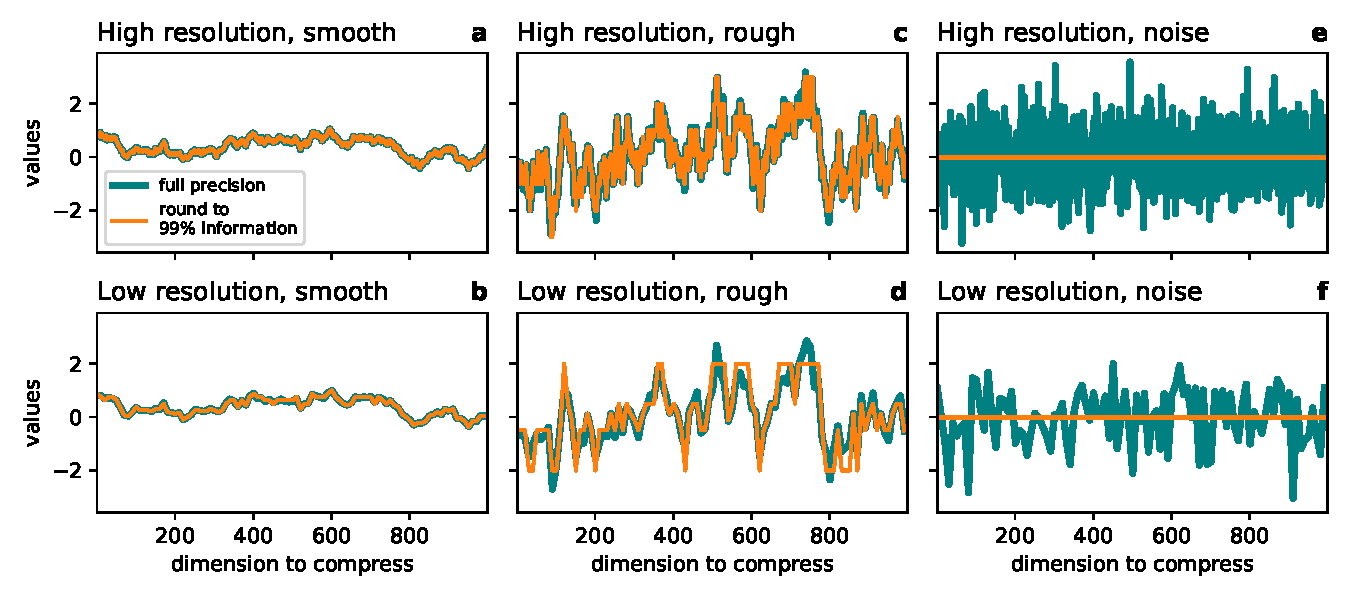
\includegraphics[width=1\textwidth]{Figures/compression/resolution_information.pdf}
	\caption{\textbf{Resolution and smoothness dependence of the information-preserving compression. a,b}
	Highly autocorrelated data (1st order auto-regressive process with correlation $r=0.999$) will have many
	mantissa bits preserved, at high and low resolution. \textbf{c,d} Many mantissa bits in data with less autocorrelation
	($r=0.95$) will be independent at low resolution and therefore rounded to zero. \textbf{e,f} All bits in random data ($r=0$)
	drawn from a standard normal distribution are fully independent so that removing the false information rounds
	this data to zero. Low resolution data (\textbf{b,d,f}) is obtained from high resolution (\textbf{a,c,e}) by subsampling every
	10th data point.}
	\label{fig:information_resolution}
\end{figure}

\begin{figure}[tbhp]
	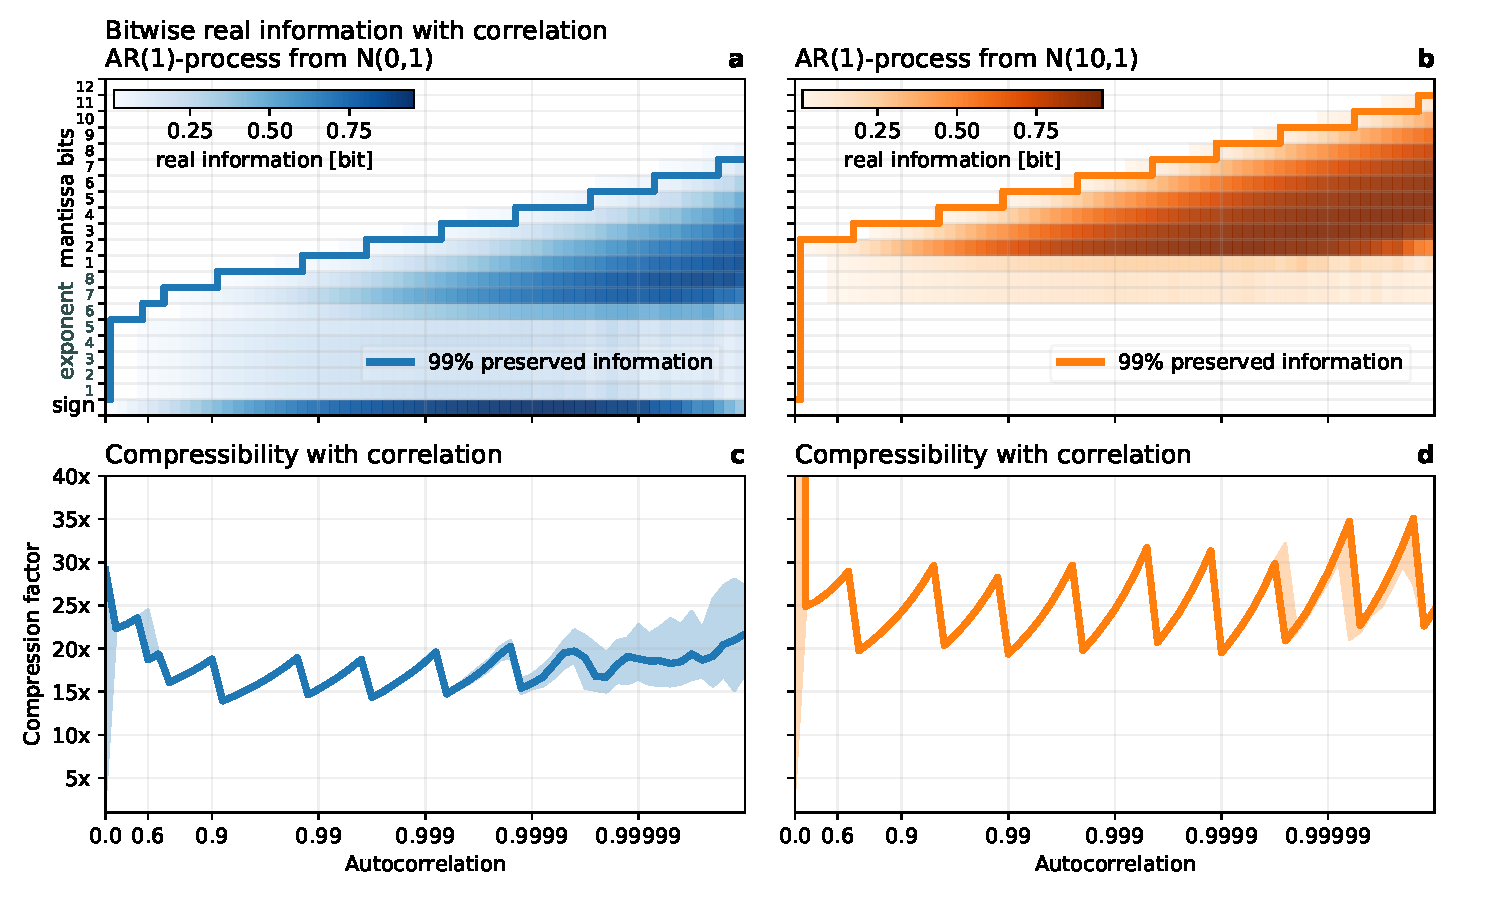
\includegraphics[width=1\textwidth]{Figures/compression/correlation_ar1.pdf}
	\caption{\textbf{Dependency of the bitwise real information and compressibility on correlation. a}
	The bitwise real information content of a first-order autoregressive process (AR(1) with Gaussian distribution N(0,1),
	i.e. with zero mean and unit variance) with varying lag-1 autocorrelation. The bits that have to be retained to preserve
	99\% of information are enclosed with a solid line. \text{b} as \textbf{a} but the AR(1) process follows a Gaussian distribution with
	a mean of 10. \textbf{c,d} Compression factors for \textbf{a,b} when preserving 99\% of information. Shading denotes the interdecile range.}
	\label{fig:information_correlation}
\end{figure}

\section{Methods: Properties of real information}
\label{sec:compression_methods_properties}

\subsection{Dependency of the bitwise real information on correlation}

The real information as defined here depends on the mutual information of bits in adjacent grid points.
Higher autocorrelation in data (meaning a higher correlation between adjacent grid points) increases the
mutual information in the mantissa bits. With higher correlation the adjacent grid values are closer,
increasing the statistical dependence of mantissa bits that would otherwise be independent at lower correlation.
Consequently, the real bitwise information content is increased and more mantissa bits have to be retained to
preserve 99\% of real information (Fig. \ref{fig:information_correlation}a and b).

The increasing number of retained mantissa bits with higher autocorrelation in data will decrease compression factors,
as it is easier to compress bits that are rounded to zero. However, a higher correlation also increases the redundancy
in bits of adjacent grid points, which favours a more efficient lossless compression. These two effects counteract and
compression factors only increase piecewise over a small range of correlations while the retained mantissa bits are
constant (Fig. \ref{fig:information_correlation}c and d). Once an additional mantissa bit has to be retained to preserve
99\% of real information, compression factors jump back down again, resulting in a sawtooth wave. Over a wide
range of typical correlation coefficients (0.5 - 0.9999) the compression factors are otherwise constant and no higher
compressibility is found with increased correlation. 

The compression factors can, however, depend on the range of values represented in binary: A shift in the mean to have
positive or negative values only means that the sign bit is unused, which increases compression factors
(compare Fig. \ref{fig:information_correlation}a with b), despite identical correlation coefficients. Although the correlation
is invariant under multiplicative scaling and addition, the bitwise information changes under addition: When the range of
values in data fits into a power of two its real information is shifted across bit positions into the mantissa bits, such that
the exponent bits are unused. This can be observed for atmospheric temperatures stored in Kelvin (within 200-330K)
where only the last exponent bit and mantissa bits contain information (Fig. \ref{fig:ensemble_information}).
Using Celsius instead shifts information from the mantissa bits into the exponent and sign bits.

\subsection{Limitations of the information-preserving compression}

The definition of real information presented here is based on the mutual information in adjacent grid points.
We therefore assume a spatial and temporal coherence of data that will come with some autocorrelation.
For vanishing autocorrelation in the data the real information content will drop to zero, as the mutual information
between bits in adjacent but independent grid points approaches zero. In this case the entire dataset is identified
as false information and consequently rounded to zero. In practice, this only occurs with data having autocorrelation
coefficients of less than 0.2 (Fig. \ref{fig:information_correlation}). If there is valuable scientific information in such
seemingly random data, then the underlying assumption that real information is identified by the mutual information
in adjacent grid points does not hold. 

Issues with the bitwise real information content can arise in data that was previously subject to lossy compression:
Linear or logarithmic quantization, for example, rounds data in linear or logarithmic space, respectively, which is not
equivalent to binary rounding in the floating-point format. Consequently, such a quantization will generally introduce
non-zero bits in the mantissa of floats when decompressed. These bits can have some statistical dependence,
appearing as artificial information induced by the quantization. Such artificial information can be observed as a
small background information (i.e. the bitwise real information is always significantly different from 0) or a reemerging
information in the last mantissa bits. In this case, the information distribution across bit positions deviates clearly from
the typical, where the information drops monotonically in the mantissa bits and becomes insignificantly different from
0 (see the examples in Fig. \ref{fig:bitinformation}, \ref{fig:information_correlation}, \ref{fig:information_error_ssim} or
\ref{fig:ensemble_information}). A solution to this quantization-induced artificial information is to apply the bitwise real
information analysis not on the decompressed floats but on the rounded integers representing the compressed data
in linear or logarithmic quantization. The bitwise real information content as defined here is independent of the binary
format and therefore can be applied to floats as well as the unsigned integers from quantization. Note that this issue
does not arise when rounding is applied in the same encoding which is also used to analyse the real information content.
In our case, using the floating-point representation for the rounding (i.e. removing the false information) the rounded
mantissa bits are always 0 which also means zero entropy when analysing the information. Applying the rounding for
floats repeatedly will have no effect beyond the first application (idempotence).

\begin{figure}[tbhp]
	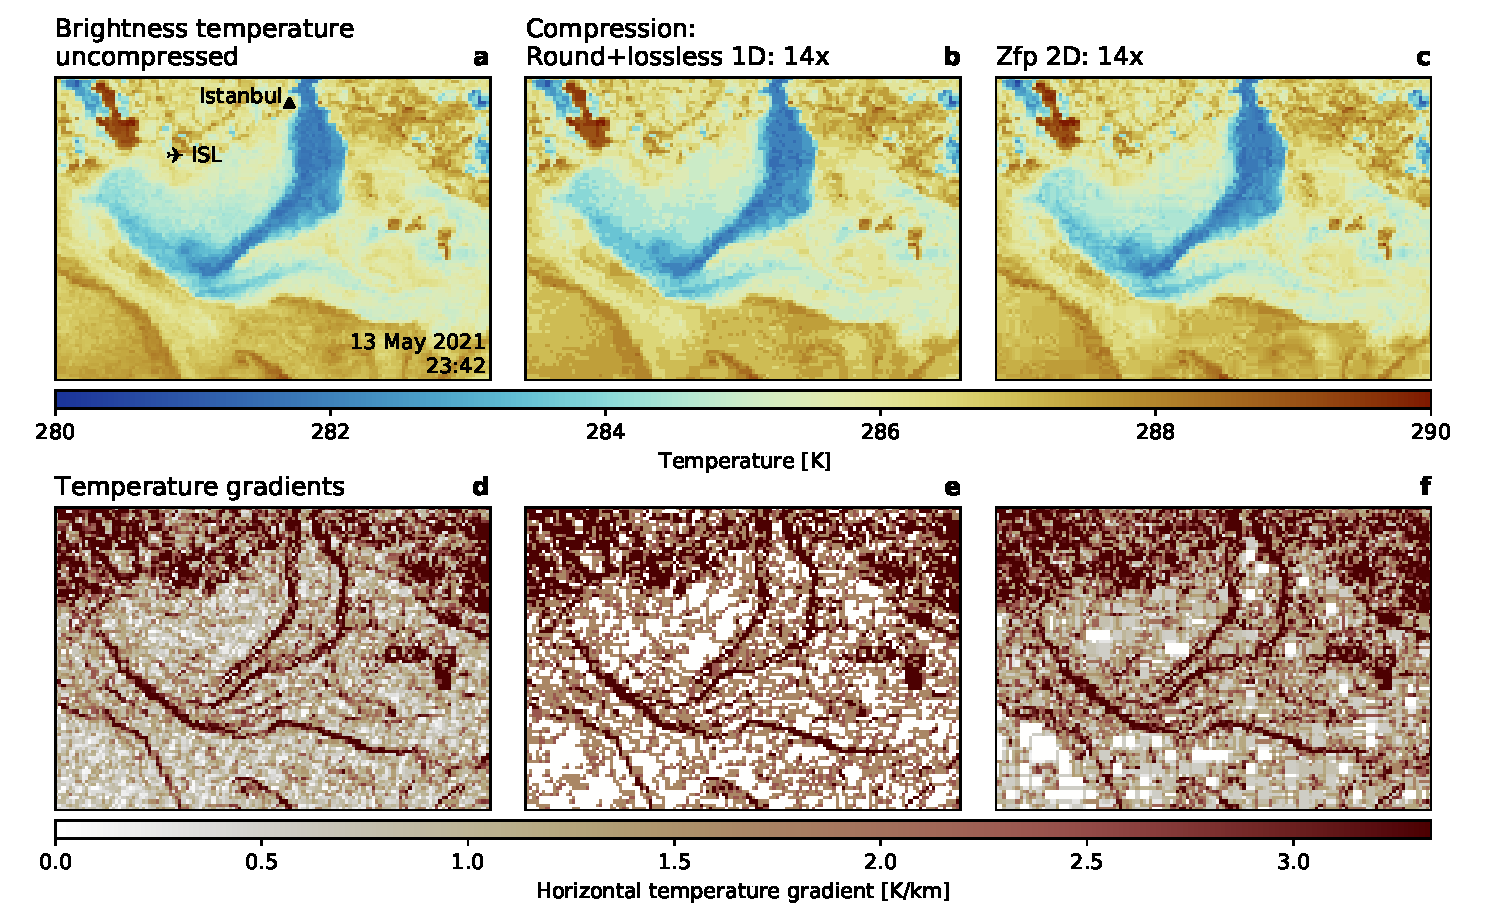
\includegraphics[width=1\textwidth]{Figures/compression/brightness_temp_grad.pdf}
	\caption{\textbf{Preservation of gradients during compression.} Compressing the brightness temperature
	of Fig. \ref{fig:brightness_temp} (VIIRS sensor aboard the satellite Suomi NPP) south of Istanbul where
	the Black Sea outflows into the Marmara Sea. Oceanic fronts with strong horizontal gradients in sea surface
	temperature are visible. \textbf{a} Brightness temperature uncompressed. \textbf{b} as \textbf{a} but compressed
	using round+lossless preserving 99\% of real information. \textbf{c} as \textbf{a} but using Zfp compression in the
	two horizontal dimensions. \textbf{d} Horizontal temperature gradient uncompressed highlighting the oceanic
	fronts from \textbf{a}. \textbf{e} as \textbf{a} but the horizontal gradient is calculated from the round+lossless
	compressed dataset as shown in \textbf{b}. \textbf{f} as \textbf{e} but using Zfp compression as shown in \textbf{c}. 
	The coarseness of the visualisation represents the resolution of the data.
	Istanbul (Hagia Sophia) and Atatürk Airport (ISL) are marked for orientation.}
	\label{fig:compression_gradients}
\end{figure}

\subsection{Preservation of gradients}

The preservation of gradients and other higher-order derivatives in data is a challenging aspect of compression.
Removing false information in data via rounding can result in identical values in adjacent grid points. Even if these values
were not identical before rounding, they may not be significantly different from each other in the sense of real and false
information. In this case, a previously weak but non-zero gradient will be rounded to zero. In other cases the rounding error
is small compared to the standard deviation of the data, such that rounding has a negligible impact on the variance as
values are independently equally likely to be round up or down.

This can be illustrated in the example of analysing oceanic fronts obtained from satellite measurements of sea surface
temperatures (Fig. \ref{fig:compression_gradients}). Identified by large horizontal gradients in temperature, the location
and strength of oceanic fronts is well preserved using compressed data. However, areas of very weak gradients can
largely vanish with round+lossless (Fig.  \ref{fig:compression_gradients}e). In this case the temperature in adjacent grid
points is insignificantly different from each other and therefore the gradient zero after the removal of false information.
Weak gradients are better preserved with Zfp compression at similar compression factors, but its block structure becomes
visible (Fig. \ref{fig:compression_gradients}f). 

\begin{figure}[tbhp]
	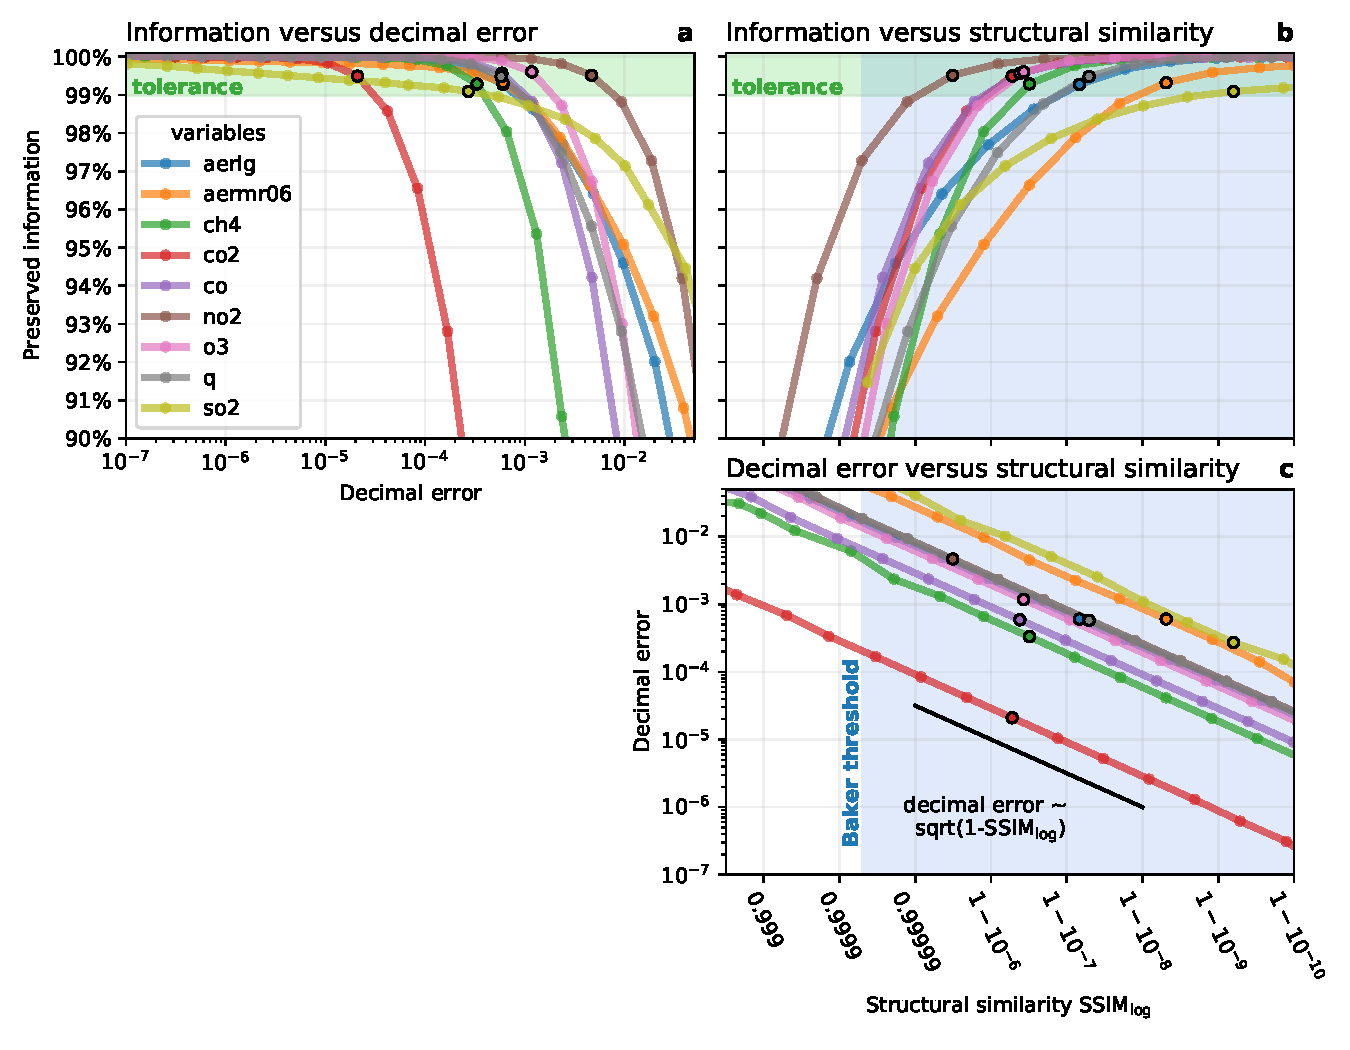
\includegraphics[width=1\textwidth]{Figures/compression/information_error_ssim.pdf}
	\caption{\textbf{The relationships between preserved information, decimal error and structural similarity for rounding within
	the information-preserving compression. a} The last 1\% of information tends to be distributed across many mantissa bits
	such that a trade-off arises where a large increase in compressibility is achieved for a small tolerance in information loss.
	The preserved information is presented as a function of the decimal error, which itself increases exponentially for
	every additional bit (small circles) that is discarded due to rounding. Denoted circles present the number of mantissa bits
	that have to be retained during compression to preserve at least 99\% of information. \textbf{b} The preserved information
	increases as a function of the structural similarity (SSIM, \cite{Wang2004}). The proposed threshold for climate data of
	SSIM=0.99995 by \cite{Baker2019} is shaded. All variables are very close or above the Baker threshold when preserving
	99\% of information. \textbf{c} The decimal error is proportional to the square root of the structural dissimilarity 1-SSIM
	for binary rounding within the information-preserving compression}
	\label{fig:information_error_ssim}
\end{figure}

\subsection{Structural similarity}

A metric to assess the quality of lossy compression in image processing is the structural similarity index measure (SSIM, \cite{Wang2004}).
For images it is based on comparisons of luminance, contrast and structure. For floating-point arrays the luminance contributions
to SSIM can be interpreted as the preservation of the mean; the contrast compares the variances and the structure compares the
correlation. The SSIM of two arrays $A,B$ of same size is defined as
	\begin{equation}
	\op{SSIM}(A,B) = \frac{(2\mu_A\mu_B + c_1)(2\sigma_{AB} + c_2)}{(\mu_A^2 + \mu_B^2 + c_1)(\sigma^2_A + \sigma^2_B + c_2)}
	\end{equation}
With $\mu_A,\mu_B$ the respective means, $\sigma^2_A,\sigma^2_B$ the respective variances and $\sigma_{AB}$ the covariance.
$c_1 = (k_1L)^2$ and $c_2 = (k_2L)^2$  are introduced to increase stability with a small denominator and $k_1 = 0.01, k_2 = 0.03$.
The dynamic range is $L = \max(\max(A),\max(B)) - \min(\min(A),\min(B))$. The SSIM is a value in $[0,1]$ where the best possible
similarity $\op{SSIM}=1$ is only achieved for identical arrays.

For rounded floating-point arrays the decimal error is proportional to the square root of the dissimilarity $1-\op{SSIM}$
(Fig. \ref{fig:information_error_ssim}c). The SSIM in this case is approximately equal to the correlation, as round-to-nearest is
bias-free (i.e. $\mu_A \approx \mu_B$) and as the rounding error is typically much smaller than the standard deviation of the data
(i.e. $\sigma_A \approx \sigma_B$). Here, we use the logarithmic SSIM, $\op{SSIM}_{\log}(A,B) = \op{SSIM}(\log(A),\log(B))$,
which is the SSIM applied to log-preprocessed data (the logarithm is applied element-wise). The usage of SSIM$_{\log}$
is motivated due to the rather logarithmic data distribution for most variables (Fig. \ref{fig:cams_histograms}),
but similar results are obtained for SSIM. The proportionality to the decimal error is unchanged when using SSIM$_{\log}$.

\cite{Baker2019} propose the SSIM as a quality metric for lossy compression of climate data52. While for image processing
SSIM > 0.98 is considered good quality, \cite{Baker2019} suggest a higher threshold of SSIM = 0.99995 for climate data compression.
The preserved information as defined here can be used as a compression quality metric similar to the SSIM. When preserving 99\%
of real information the SSIM$_{\log}$ is also above the Baker threshold (Fig. \ref{fig:information_error_ssim}b), reassuring that our
threshold of 99\% preserved real information is reasonable. In general, the preserved information is a monotonic function of the
structural similarity SSIM (or SSIM$_{\log}$) for rounded floating-point arrays, further supporting the usage of preserved
information as a metric for data compression. 

\section{Methods: Compression}
\label{sec:compression_methods_compression}

\subsection{Linear and logarithmic quantization}

The $n$-bit linear quantization compression for each element $a$ in an array $A$ is
	\begin{equation}
	\tilde{a} = \op{round} \left( 2^{n-1} \frac{a - \min(A)}{\max(A) - \min(A)} \right)
	\end{equation}
with $\op{round}$ a function that rounds to the nearest integer in $0,...,2^{n-1}$. Consequently, every compressed element $\tilde{a}$
can be stored with $n$ bits. The $n$-bit logarithmic quantization compression for every element $a\geq0$ in $A$ is
	\begin{equation}
	\tilde{a} = \begin{cases} 0 \quad &\text{if } a = 0, \\
	\text{round}\left( c + \Delta^{-1}\log(a) \right) + 1 \quad &\text{else.} \end{cases}
	\end{equation}
which reserves the bit pattern zero to encode 0. The logarithmic spacing is
	\begin{equation}
	\Delta = \frac{\log(\max(A)) - \log(\min^+(A))}{2^{n}-2}
	\end{equation}
The constant $c = 1/2 - \Delta^{-1}\log(\text{min}^+(A)(\exp(\Delta)+1)/2)$ is chosen to implement round-to-nearest in linear space
instead of in logarithmic space, for which $c=-\Delta^{-1}\log(\text{min}^+(A))$. The function $\min^+(A)$  is the minimum of all
positive elements in $A$.

\subsection{Lossless compression}

We use Zstandard as a default lossless algorithm for the round+lossless method. Zstandard is a modern compression algorithm
that combines many techniques to form a single compressor with tunable 22 compression levels that allow large trade-offs between
compression speed and factors \citep{Skibinski2020,Collet2020}. Here, we use compression level 10, as it presents a reasonable
compromise between speed and size. Zstandard outperforms other tested algorithms (deflate, LZ4, LZ4HC and Blosc) in our
applications and is also found to be among the best in the lzbench compression benchmark \citep{Skibinski2020} and other studies
have focused on comparisons \citep{Delaunay2019}. Lossless compressors
are often combined with reversible transformations that preprocess the data. The so-called bitshuffle transposes an array on the
bit-level, such that bit positions (e.g. the sign bit) of floating-point numbers are stored next to each other in memory. Another example
is the bitwise XOR-operation \citep{Pelkonen2015a} with the preceding floating-point value, which sets subsequent bits that are identical
to 0. Neither bitshuffle nor XOR significantly increased the compression factors in our applications.

\begin{figure}[tbhp]
	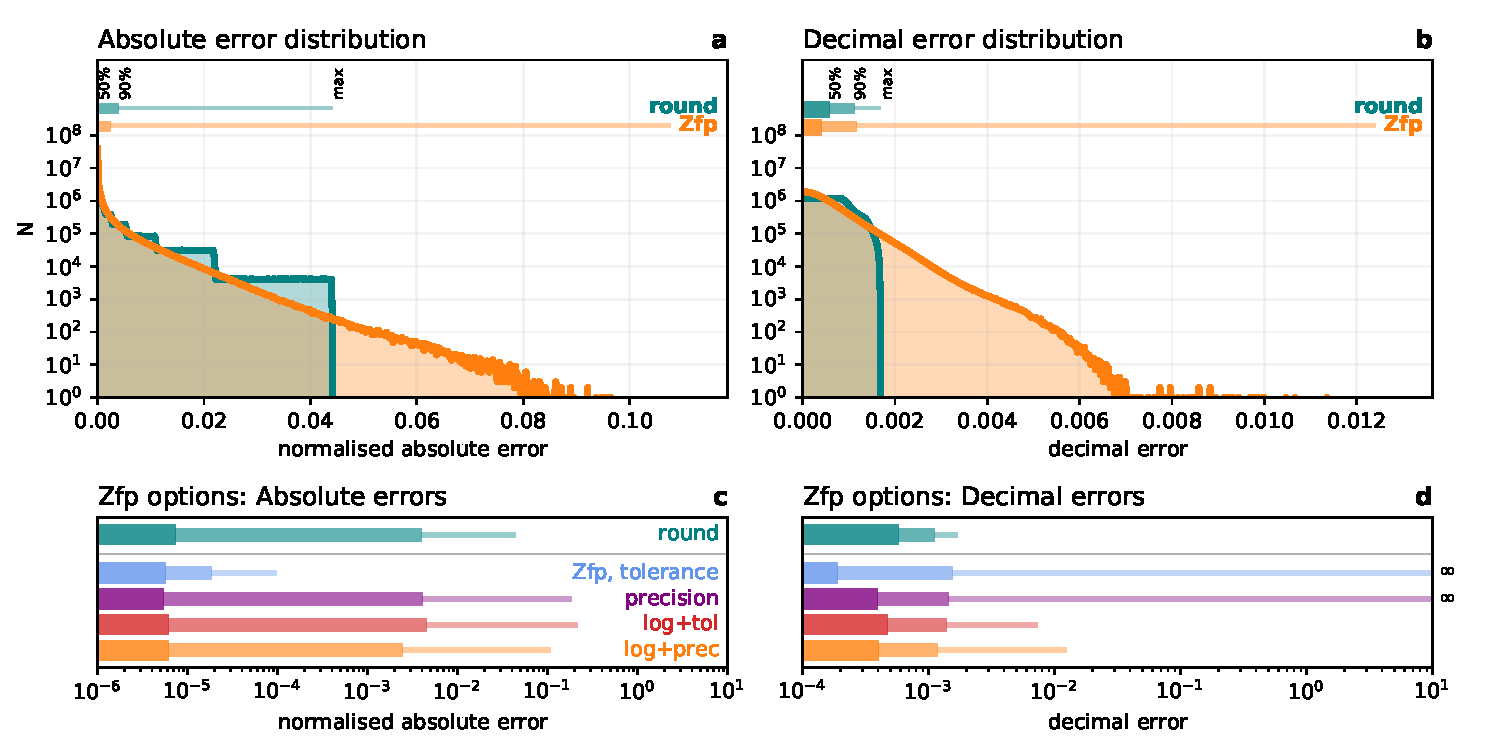
\includegraphics[width=1\textwidth]{Figures/compression/error_distributions.pdf}
	\caption{\textbf{Error distribution of binary rounding compared to Zfp compression.} 
	IEEE round-to-nearest and Zfp compression of water vapour (specific humidity) in the
	three spatial dimensions. \textbf{a, c} normalised absolute errors \textbf{b, d} decimal errors.
	7 mantissa bits are retained for rounding corresponding to 99\% preserved information.
	The precision parameter of Zfp is chosen to yield median errors that are at least as small
	as those obtained by rounding. \textbf{c, d} Zfp via specifying tolerance (tol) or precision (prec)
	with and without log-preprocessing. Maximum decimal errors that reached infinity in \textbf{d}
	due to sign changes are marked.}
	\label{fig:compression_error_distribution}
\end{figure}

\subsection{Matching retained bits to Zfp's precision}

The Zfp compression algorithm divides a $d$-dimensional array into blocks of size $4^d$ to exploit correlation
in every dimension of the data. Within each block a transformation of the data is applied with specified absolute
error tolerance or precision, which bounds a local relative error. We use Zfp in its precision mode, which offers
discrete levels to manually adjust the retained precision. Due to the rather logarithmic distribution of CAMS data
(Fig. \ref{fig:cams_histograms}), a log-preprocessing of the data is applied to prevent sign changes (including a flushing to zero) within
the compression. The error introduced by Zfp is approximately normally distributed and therefore usually yields
higher maximum errors compared to round-to-nearest in float arithmetic, although median errors are comparable.
In order to find an equivalent error level between the two methods, we therefore choose the precision level of Zfp
to yield median absolute and decimal errors that are at least as small as those from rounding.

This method is illustrated in Fig. \ref{fig:compression_error_distribution} in more detail: Errors introduced from
round-to-nearest for floats have very rigid error bounds, the majority of errors from Zfp compression are within
these bounds when matching median errors. However, given the normal distribution of errors with Zfp, there will
be a small share of errors that is beyond the bounds from round-to-nearest. Using the precision mode of Zfp and
log-preprocessed data bounds these maximum errors well (Fig. \ref{fig:compression_error_distribution}c and d).

\begin{figure}[tbhp]
	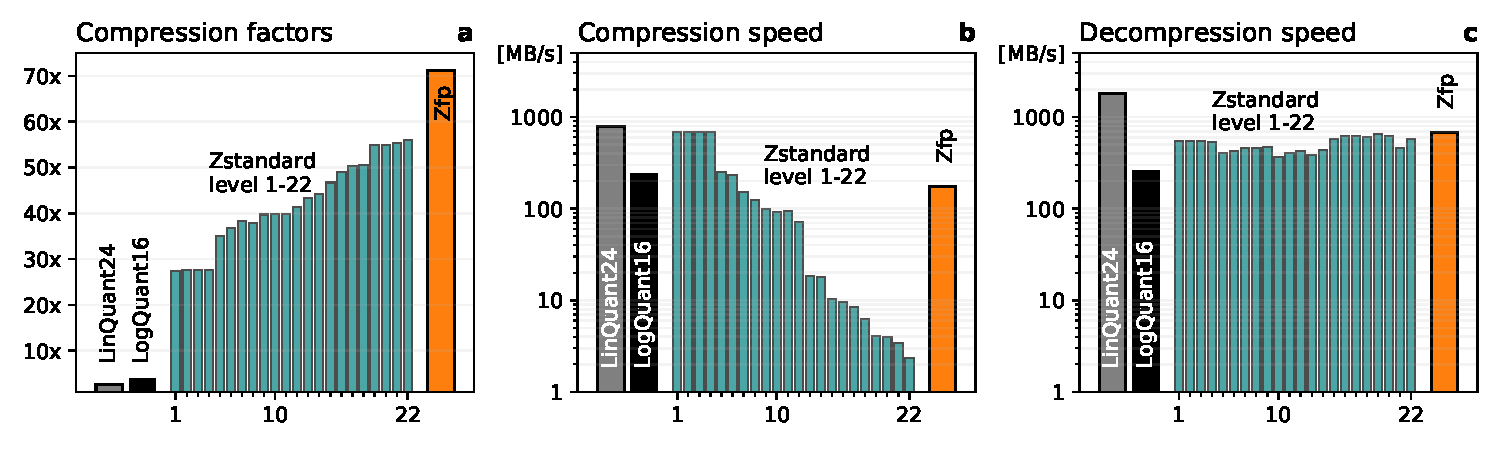
\includegraphics[width=1\textwidth]{Figures/compression/compression_speed.pdf}
	\caption{\textbf{Compressor performances.} 
	Compressing water vapour (specific humidity, variable code q) (3 mantissa bits retained, as in Fig.
	\ref{fig:map_roundlossless_zfp}) with 24-bit linear quantization (LinQuant24), 16-bit logarithmic quantization
	(LogQuant16), round+lossless (Zstandard, compression level 1-22) and Zfp (precision-mode,
	including log-preprocessing): \textbf{a} Compression factors, \textbf{b} compression speed, \textbf{c}
	decompression speed. Timings are single-threaded on an Intel Core\texttrademark~i7 (Kaby Lake) and do not include the writing to disk.}
	\label{fig:compression_speed}
\end{figure}

\subsection{Compressor performances}

Although different compressors and their performance are not within the central focus of this study, we analyse
the compression and decompression speeds as a sanity check (Fig. \ref{fig:compression_speed}). In order to
find a data compression method that can be used operationally, a certain minimum data throughput should be achieved.
The current 24-bit linear quantization method reaches compression speeds of almost 800 MB/s single-threaded on an
Intel Core\texttrademark~i7 (Kaby Lake) CPU in our application, excluding writing to disk. For the logarithmic quantization,
this decreases to about 200 MB/s due to the additional evaluation of a logarithm for every value. For Zstandard the user
can choose between 22 compression levels, providing a trade-off between the compression speed (highest for level 1)
and the compression factor (highest for level 22). Compression speed reduces from about 700 MB/s at compression level 1
to 2 MB/s at level 22 (Fig. \ref{fig:compression_speed}b), such that for high compression factors about a thousand cores
would be required in parallel to compress in real time the 2GB/s data production at ECMWF. For Zstandard at compression
level 10 speeds of at least 100MB/s are achieved, but at the cost of about 50\% larger file sizes. We use compression level
10 throughout this study as a compromise. The decompression speed is independent of the level (Fig. \ref{fig:compression_speed}c).
The additional performance cost of binary rounding is with 2 GB/s negligible. Zfp reaches compression speeds of about 200 MB/s
(single-threaded, including the log-preprocessing) in our application, enough to compress ECMWF’s data production in real
time with a small number of processors in parallel.

\begin{figure}[tbhp]
	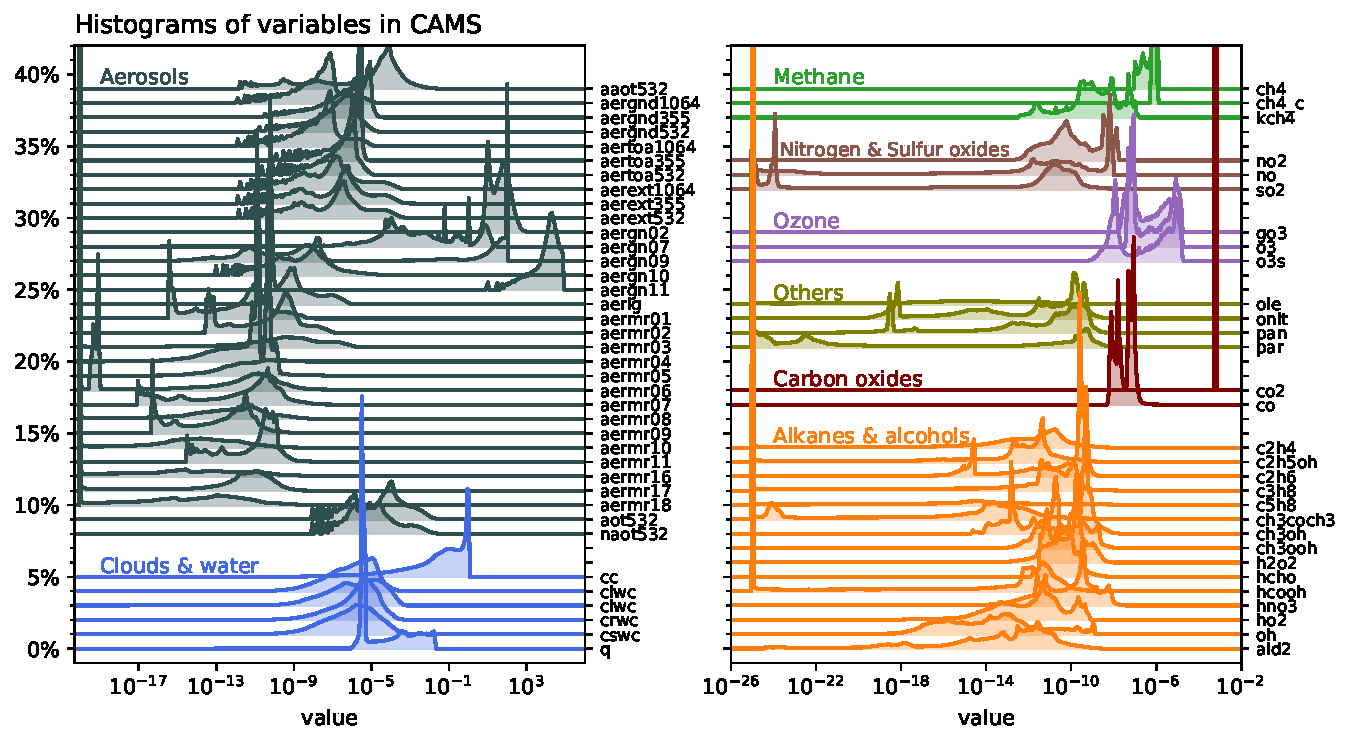
\includegraphics[width=1\textwidth]{Figures/compression/histograms.pdf}
	\caption{\textbf{Statistical distributions of all variables in CAMS.}
	Histograms use a logarithmic binning and are staggered vertically for clarity.
	The variable abbreviations are explained in Table \ref{tab:cams_abbreviations}.}
	\label{fig:cams_histograms}
\end{figure}

\begin{figure}[tbhp]
	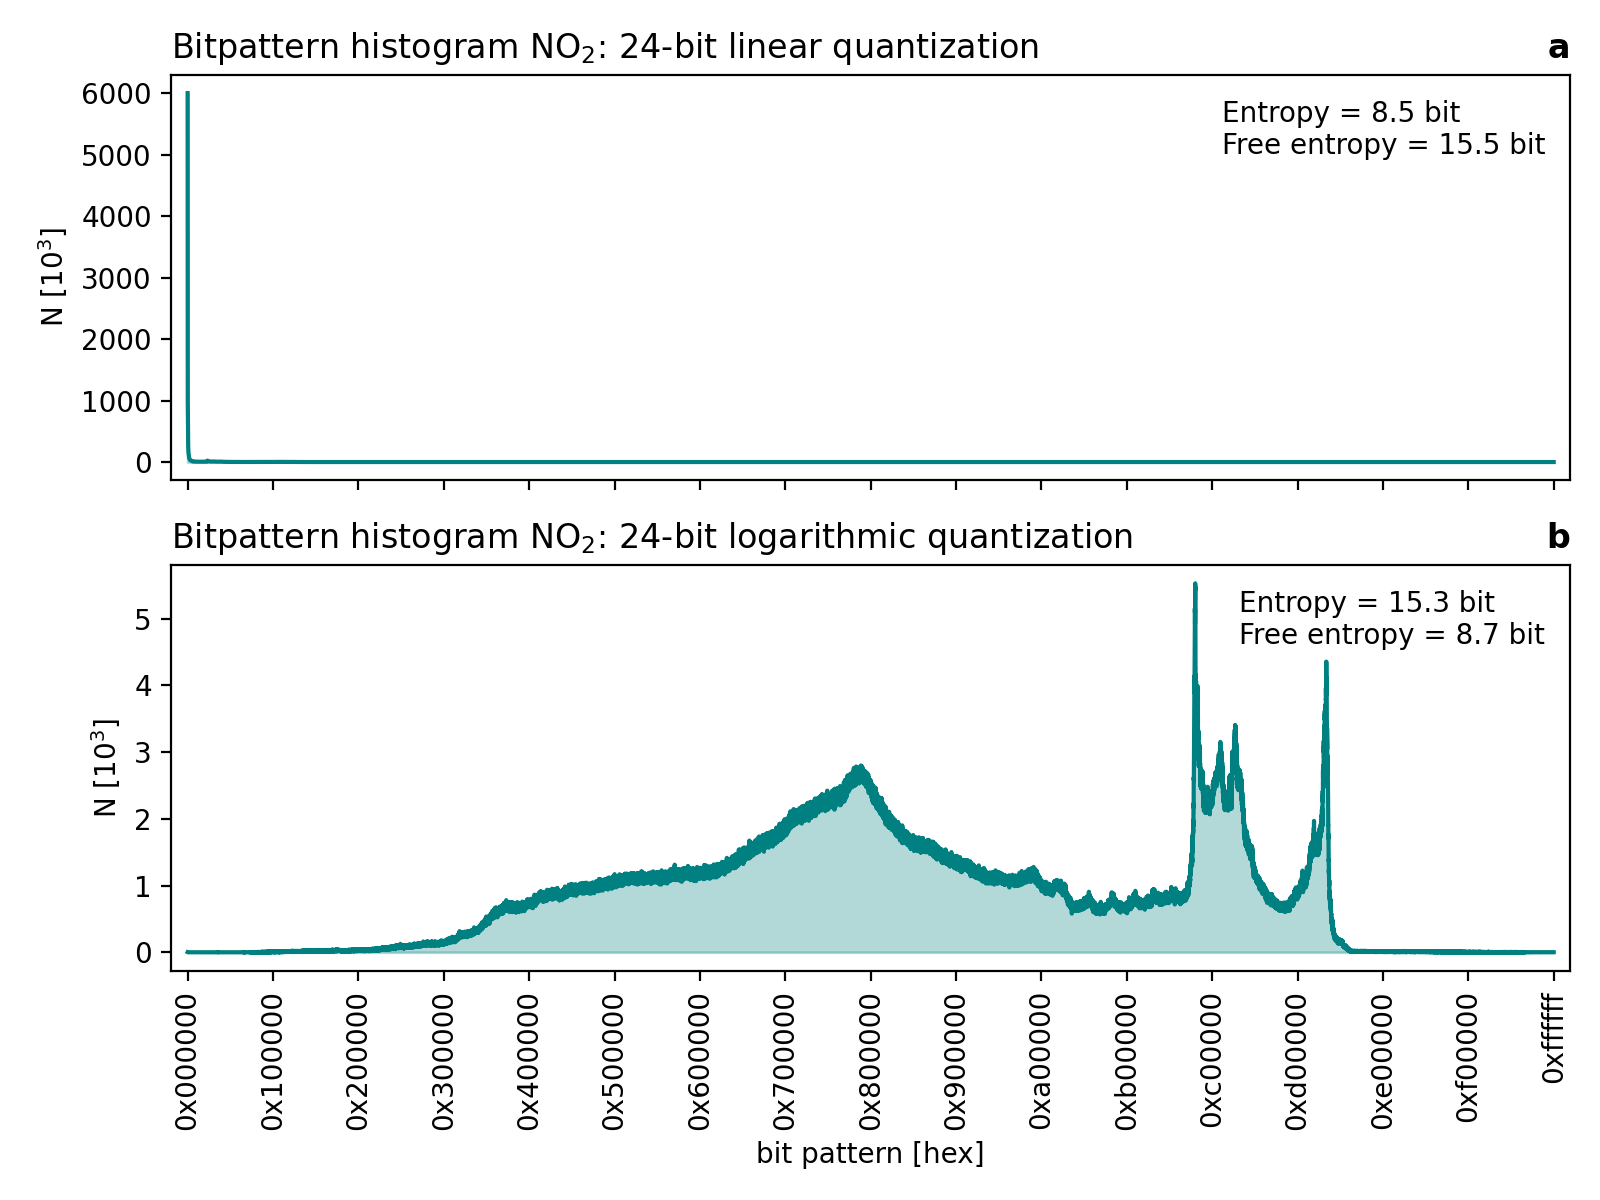
\includegraphics[width=1\textwidth]{Figures/compression/bitpattern_hist.png}
	\caption{\textbf{Bitpattern histogram for linear and logarithmic quantization. a}
	Linear 24-bit quantization and \textbf{b} 24-bit logarithmic quantization of nitrogen dioxide NO\textsubscript{2} mixing ratio [kg/kg].
	All grid points and all vertical levels are used, consisting of $5.6 \cdot 10^7$ values with a range of $2 \cdot 10^{-14}$ to
	$2 \cdot 10^{-7}$ kg/kg. Bitpatterns are denoted in 24-bit hexadecimal. The free entropy is the difference between the
	available 24 bit and the bitpattern entropy and quantifies the number of effectively unused bits.}
	\label{fig:compression_bitpattern_hist}
\end{figure}

\section{Results}
\label{sec:compression_results}
\subsection{Drawbacks of current compression methods}

The Copernicus Atmospheric Monitoring Service (CAMS, \cite{Inness2019}) is performing operational predictions with an extended
version of the Integrated Forecasting System IFS, the global atmospheric forecast model implemented by ECMWF.
CAMS includes various atmospheric composition variables, like aerosols, trace and greenhouse gases that are
important to monitor global air quality. The system monitors for example the spread of volcanic eruptions or
emissions from wildfires. Most variables in CAMS have a multi-modal statistical distribution, spanning many
orders of magnitude (Fig. \ref{fig:cams_histograms}).

The current compression technique for CAMS is the linear quantization, widely used in the weather and climate
community through the data format GRIB2 \citep{WMO2003}. CAMS uses the 24-bit version, which encodes values
in a data array with integers from $0$ to $2^{24}-1$. These 24-bit unsigned integers represent values linearly distributed
in the min-max range. Unused sign or exponent bits from the floating-point representation are therefore avoided and
some of the trailing mantissa bits are discarded in quantization. Choosing the number of bits for quantization
determines the file size, but the precision follows implicitly, leaving the required precision or amount of preserved
information unassessed.

Although linear quantization bounds the absolute error, its linear distribution is unsuited for most variables in CAMS:
Many of the available 24 bits are effectively unused as the distribution of the data and the quantized values match
poorly (Fig. \ref{fig:compression_bitpattern_hist}). Alternatively, placing the quantized values logarithmically in the
min-max range better resolves the data distribution. As floating-point numbers are already approximately logarithmically
distributed, this motivates compression directly within the floating-point format, which is also used for calculations in a
weather or climate model and post-processing.

\begin{figure}[tbhp]
	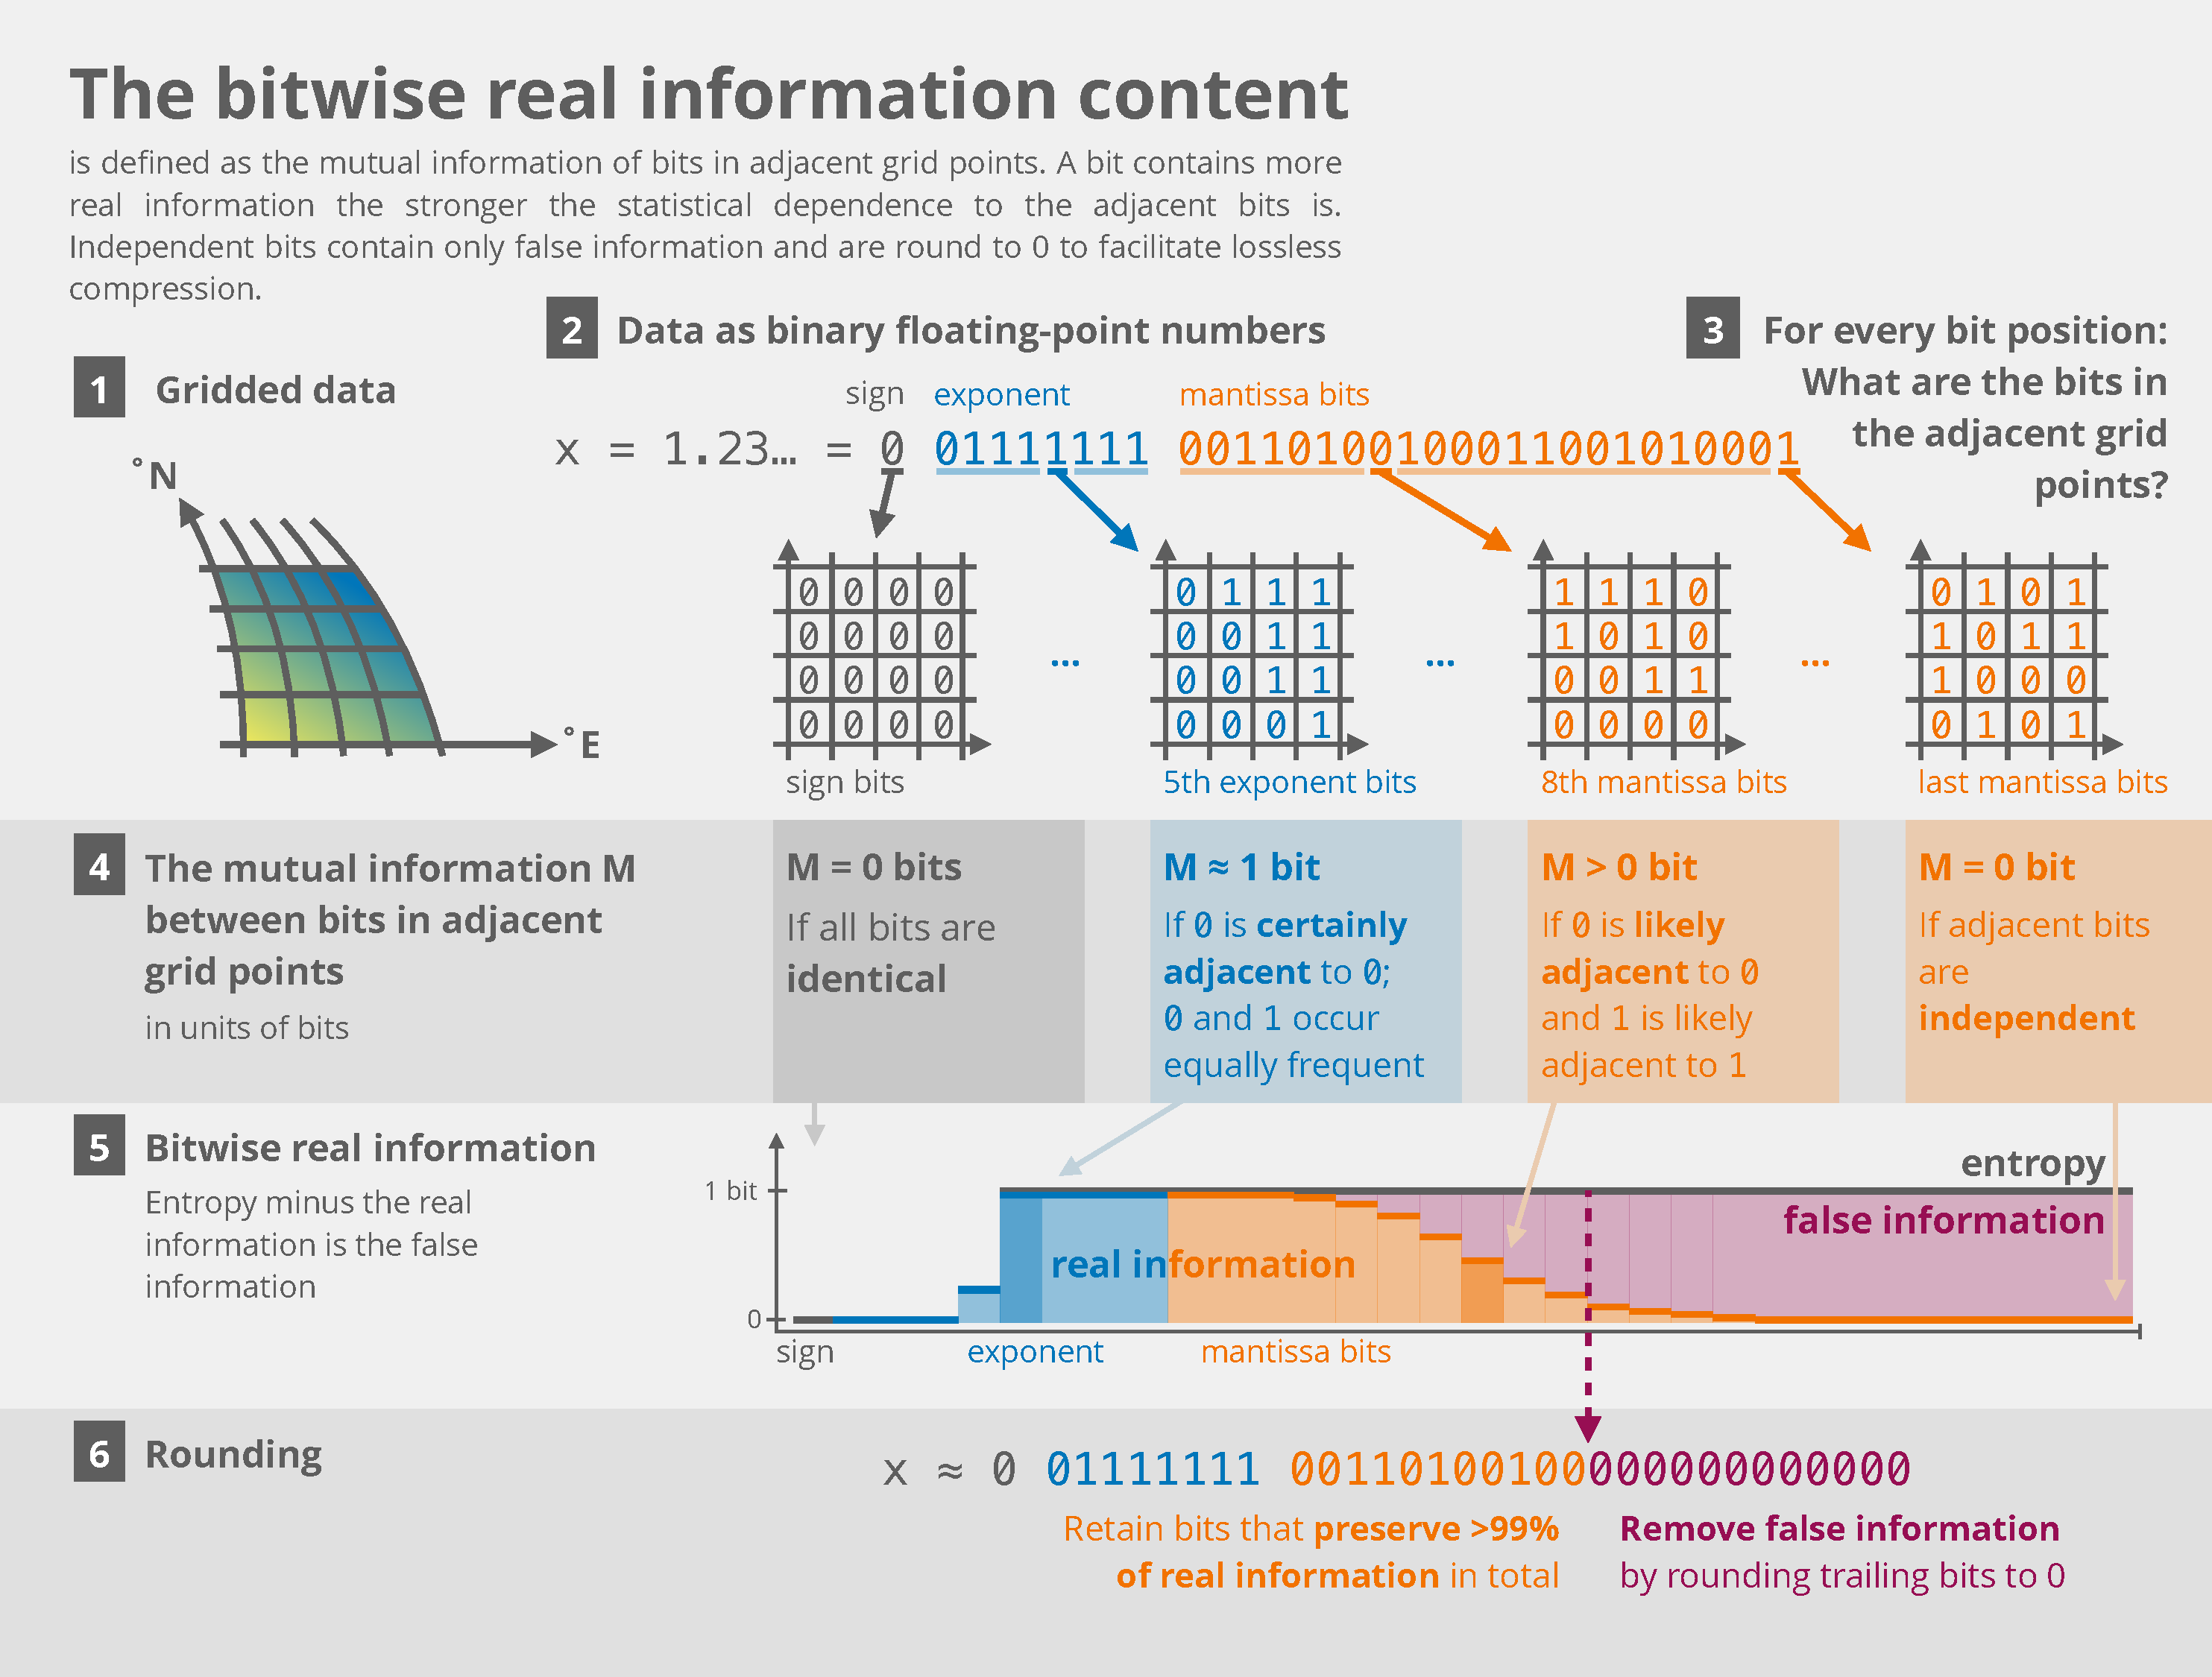
\includegraphics[width=1\textwidth]{Figures/compression/infograph_cut.pdf}
	\caption{\textbf{The bitwise real information content explained schematically.}}
	\label{fig:infograph}
\end{figure}

\begin{figure}[tbhp]
	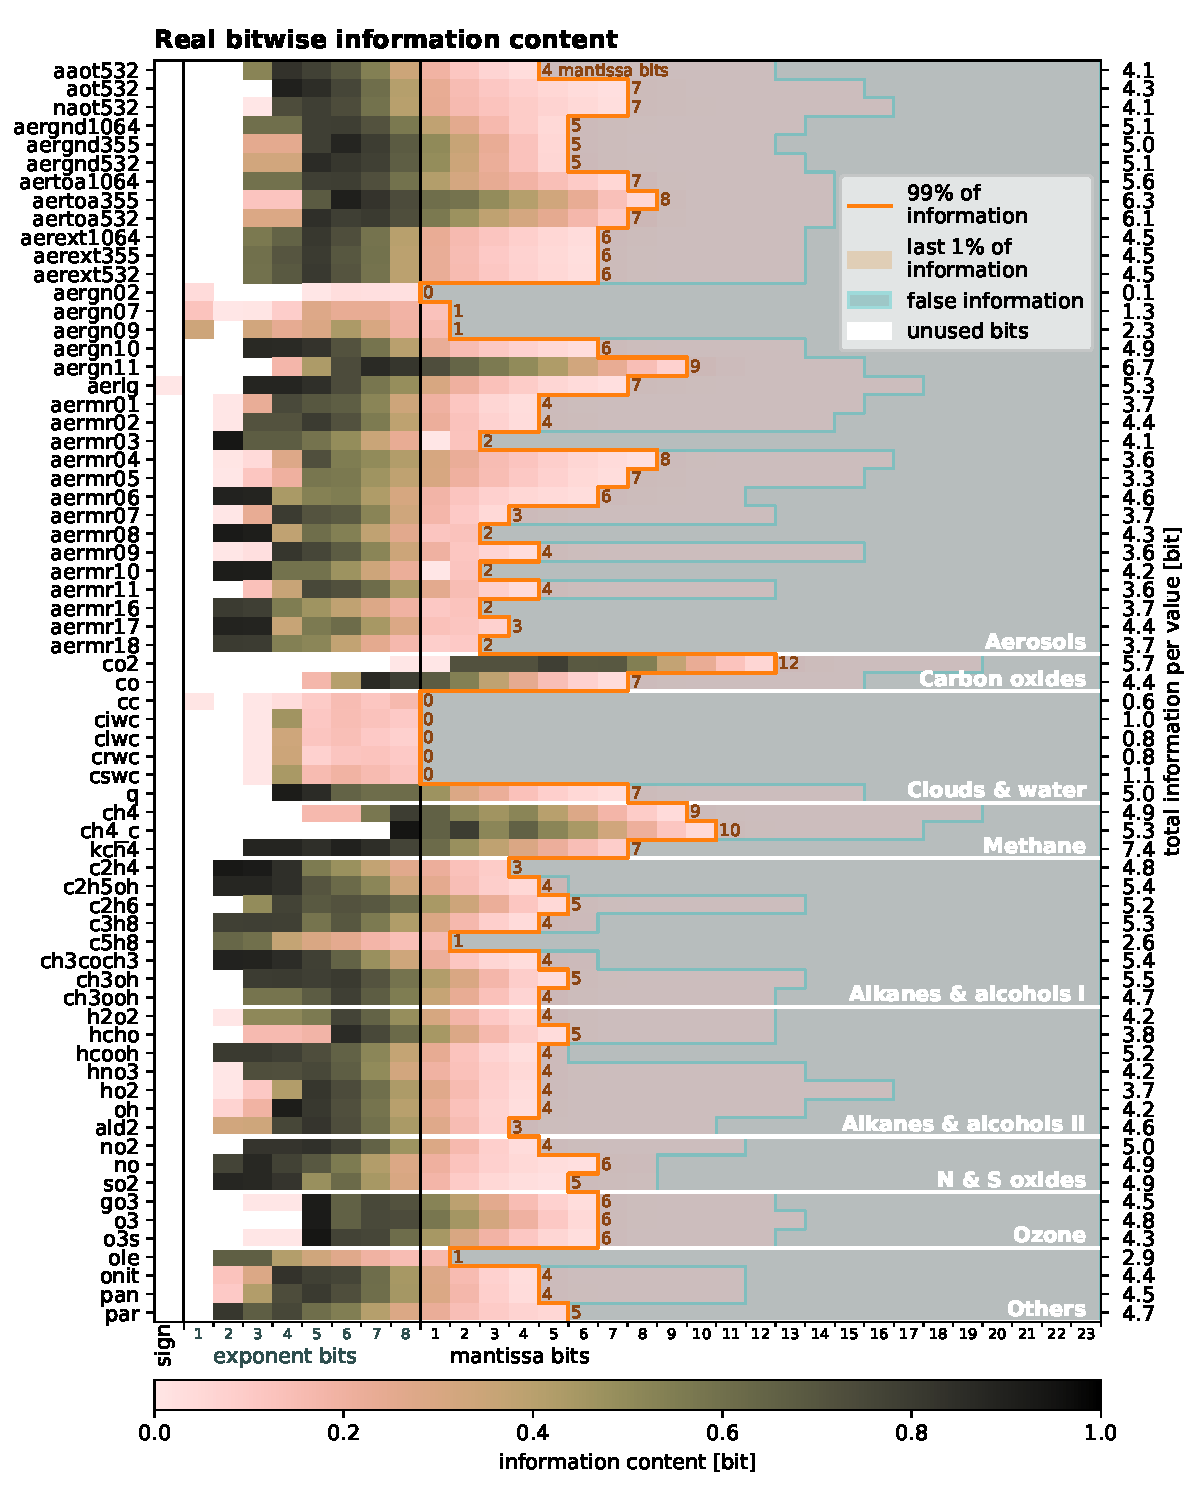
\includegraphics[width=1\textwidth]{Figures/compression/bitinformation.pdf}
	\caption{\textbf{Bitwise real information content for all variables in CAMS.} 
	The real information is calculated in all three spatial dimensions, revealing false information
	and unused bits, using the 32-bit encoding of single-precision floats. The bits that should be
	retained to preserve 99\% of real information are enclosed in orange. Bits without any real
	information are shaded in grey-blue. The sum of the real information across bit positions
	per variable is the total information per value. Variable abbreviations are explained in Table
	\ref{tab:cams_abbreviations}.}
	\label{fig:bitinformation}
\end{figure}

\subsection{Bitwise real information content}

Many of the trailing mantissa bits in floating-point numbers occur independently and at similar probability,
i.e. with high information entropy \citep{Kleeman2011,Jeffress2017}. These seemingly random bits are
incompressible \citep{MacKay2003a,Ziv1977,Huffman1952}, reducing
the efficiency of compression algorithms. However, they probably also contain a vanishing amount of real
information, which has to be analysed to identify bits with and without real information. The former should
be conserved while the latter should be discarded to increase compression efficiency.

We define the bitwise real information content as the mutual information
\citep{Shannon1948,MacKay2003a,Schreiber2000,Kraskov2004,Pothapakula2019,DelSole2004} of bits in
adjacent grid points (Fig. \ref{fig:infograph}). A bit contains more real information the stronger the statistical
dependence to the adjacent bits is. Bits without real information are identified when this dependence is
insignificantly different from zero and we regard the remaining entropy in these bits as false information.
The adjacent bit can be found in any of the dimensions of the data, e.g. in longitude, time or in the ensemble
dimension. However, always the same bit position is analysed, e.g. the dependence of the first mantissa bit
with other first mantissa bits in adjacent grid points. 

In general, this analysis can be applied to any $n$-dimensional gridded data array when its adjacent elements
are also adjacent in physical space, including structured and unstructured grids. However, data without spatial
or temporal correlation at the provided resolution will be largely identified as false information due to the
independence of adjacent grid points (Fig. \ref{fig:information_resolution} and \ref{fig:information_correlation}).
If valuable scientific information is present in such seemingly random data, then the bitwise real information
content as defined here is unsuited. 

\cite{Jeffress2017} formulate the bitwise information content for simple chaotic systems, assuming an
inherent natural uncertainty which had to be defined. Their approach aims to enable reduced precision
simulations on inexact hardware. Here, we reformulate the bitwise real information as the mutual information
in adjacent grid points for the application in climate data compression. The quantization in the floating-point
representation is used as an uncertainty, such that no additional assumption on the uncertainty of the underlying
data has to be made. While most data compression techniques leave the choice of the retained precision to the user,
the analysis here automatically determines a precision from the data itself based on the separation of real and
false information bits.     

Many exponent bits of the variables in CAMS have a high information content (Fig. \ref{fig:bitinformation}),
but information content decreases to zero within the first mantissa bits for most variables.
Exceptions occur for variables like carbon dioxide (CO\textsubscript{2}) with mixing ratios varying in a very
limited range of 0.5-1.5 mg/kg (equivalent to about 330-990ppmv) globally. Due to the limited range,
most exponent bits are unused and the majority of the real information is in mantissa bits 2 to 12.

The sum of real information across all bit positions is the total information per value, which is less than 7 bits for
most variables. Importantly, the last few percent of total information is often distributed across many mantissa bits.
This presents a trade-off where for a small tolerance in information loss many mantissa bits can be discarded,
resulting in a large increase in compressibility (Fig. \ref{fig:information_error_ssim}a). 
Aiming for 99\% preserved information is found to be a reasonable compromise.

\begin{figure}[tbhp]
	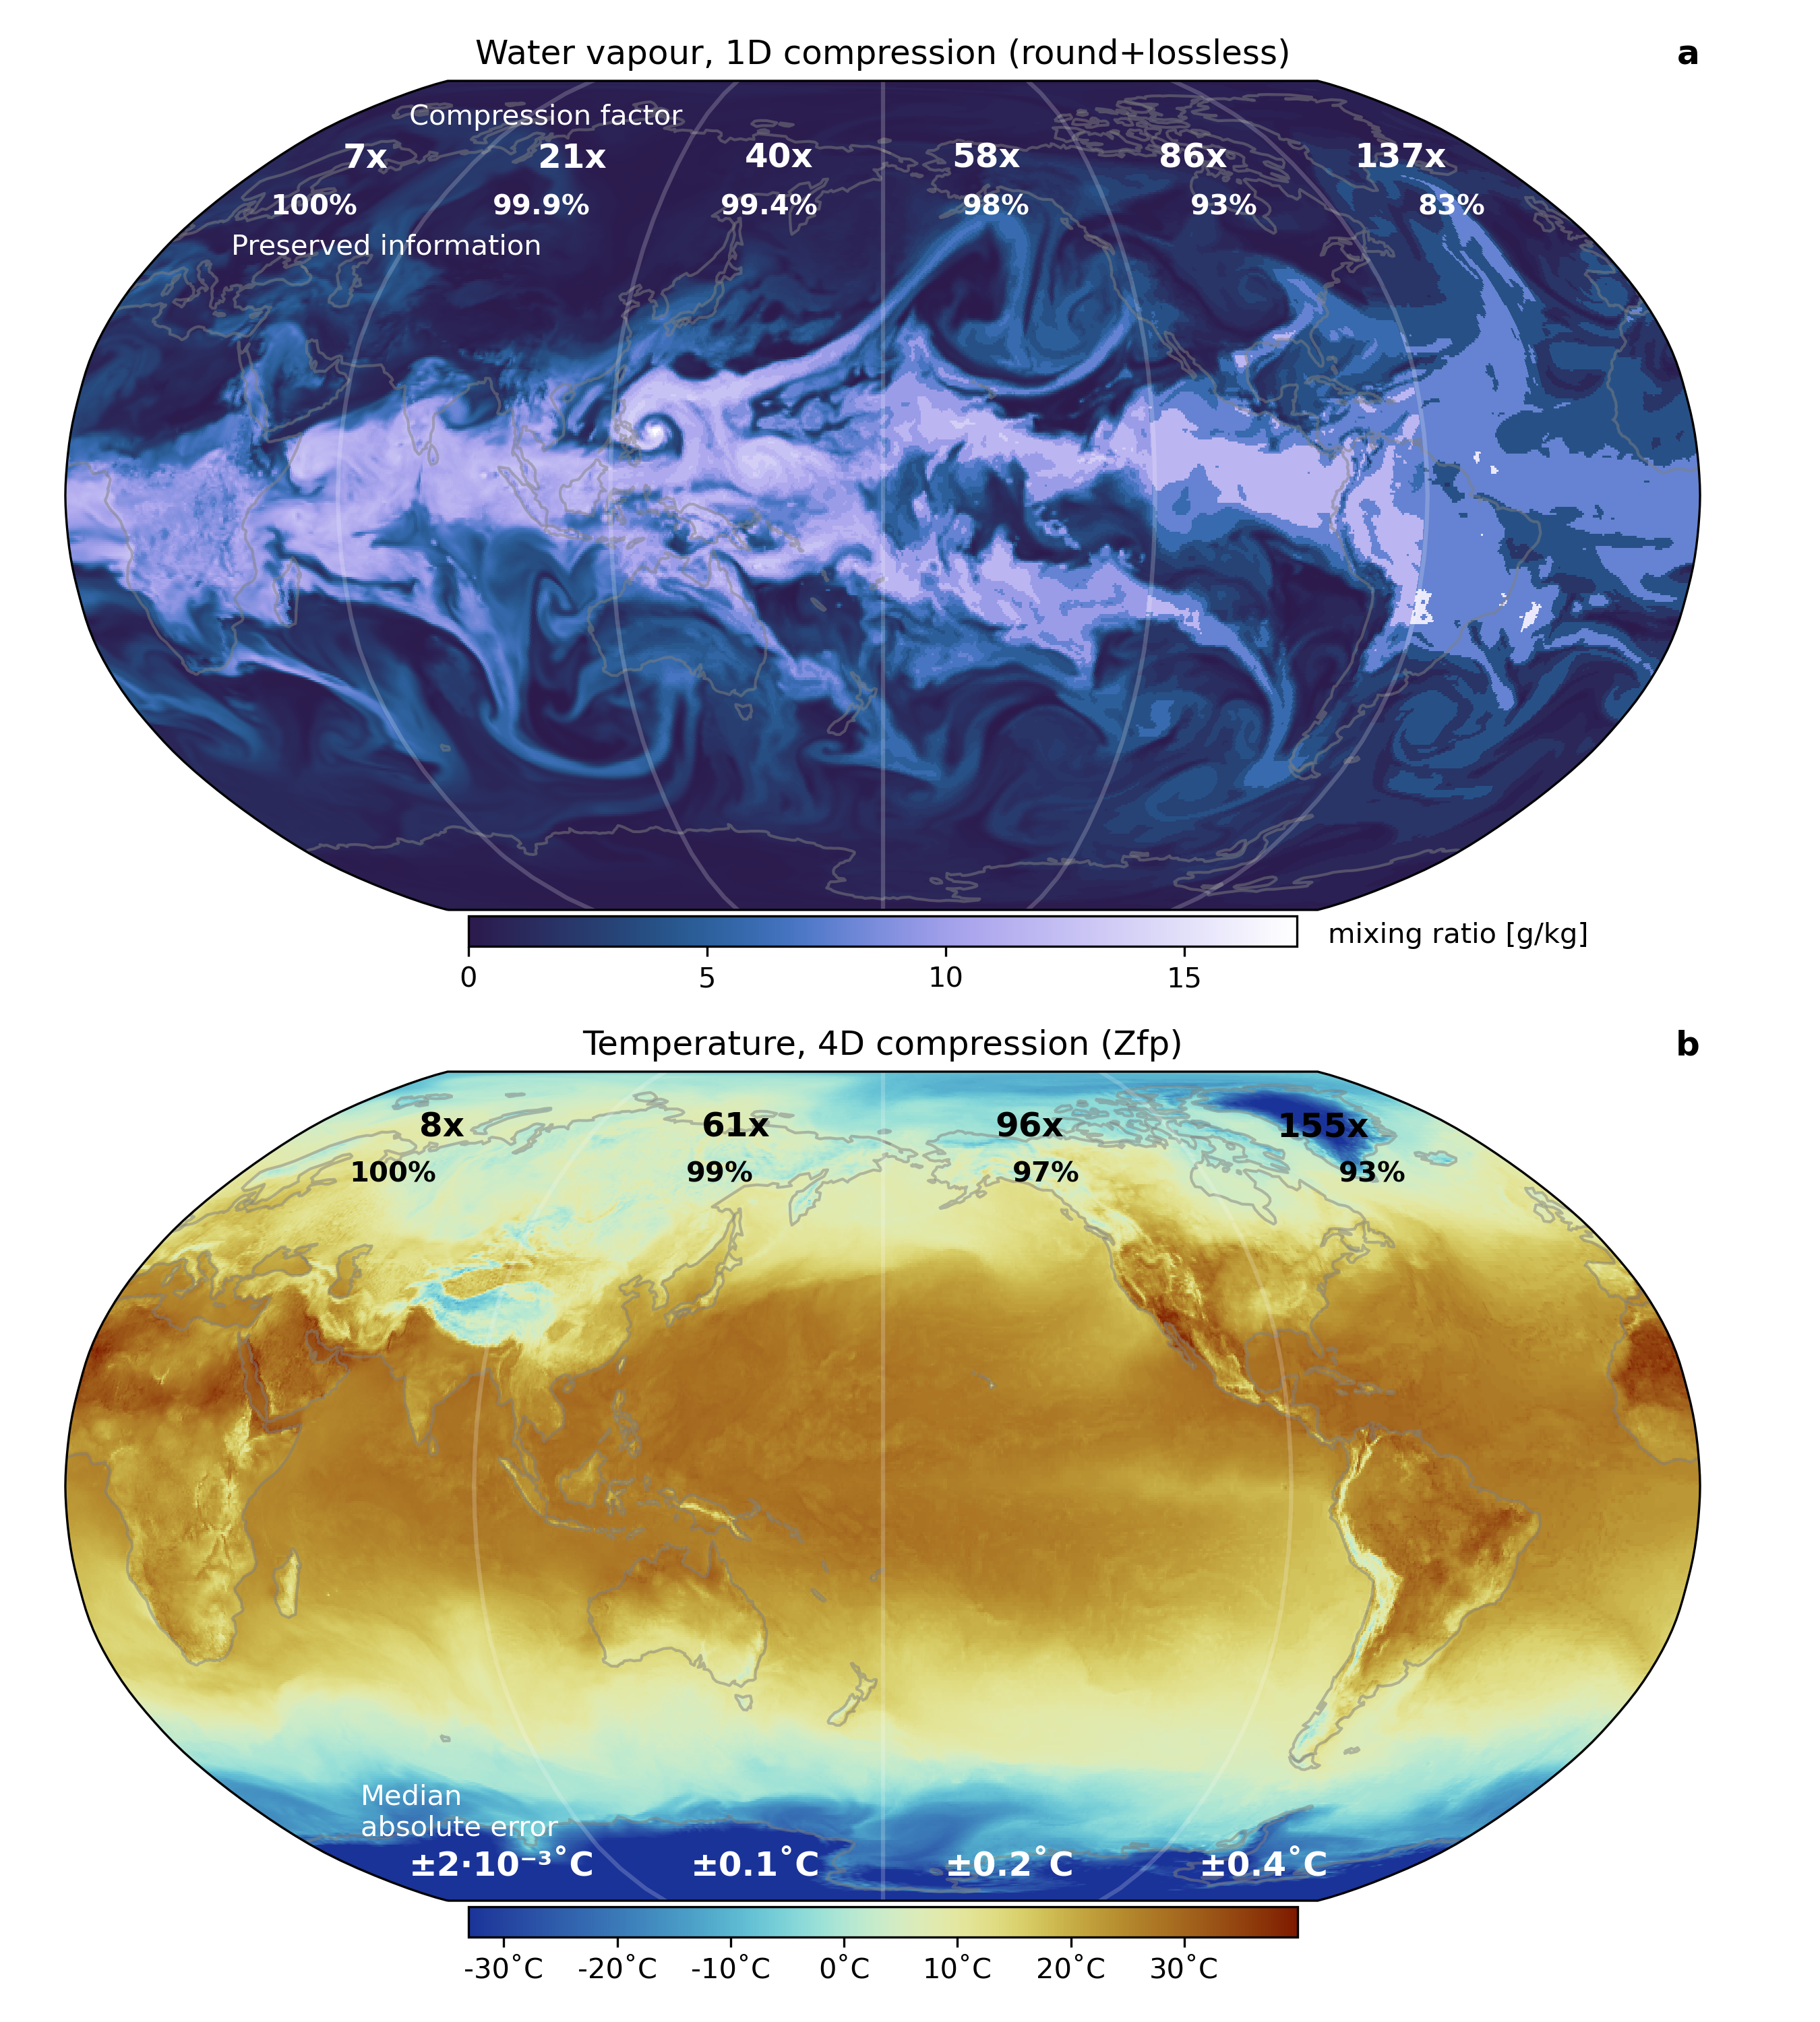
\includegraphics[width=1\textwidth]{Figures/compression/map_water_temp.png}
	\caption{\textbf{Compression at various levels of preserved information. a}
	Water vapour (specific humidity) compressed in the longitudinal dimension. 
	The vertical level shown is at about 2 km geopotential altitude, but compression 
	factors include all vertical levels. \textbf{b} Surface temperature compressed in the
	four space-time dimensions at various levels of preserved information with compression
	algorithm Zfp. Compression factors are relative to 64-bit floats.}
	\label{fig:map_roundlossless_zfp}
\end{figure}

\subsection{Compressing only the real information}

Based on the bitwise real information content, we suggest a new strategy for data compression of climate variables:
First, we diagnose the real information for each bit position. Afterwards, we round bits with no significant real information
to zero, before applying lossless data compression. This allows us to minimise information loss but to maximise the
efficiency of compression algorithms.

Bits with no or only little real information (but high entropy) are discarded via binary round-to-nearest as defined in the
IEEE-754 standard (see section \ref{sec:roundnearest}, \cite{IEEE1985}). This rounding mode is bias-free and therefore
will ensure global conservation of quantities important in climate model data. Rounding removes the incompressible false
information and therefore increases compressibility. While rounding is irreversible for the bits with false information, the
bits with real information remain unchanged and are bitwise reproducible after decompression. Both the real information
analysis and the rounding mode are deterministic, also satisfying reproducibility.

Lossless compression algorithms can be applied efficiently to rounded floating-point arrays (the \emph{round+lossless} method).
Many general-purpose lossless compression algorithms are available
\citep{Ziv1977,Ziv1978,Huffman1952,Delaunay2019,Deutsch1996,Skibinski2020,Alted2010,Collet2020}, which are based on
dictionaries and other statistical techniques to remove redundancies. Most algorithms operate on bitstreams and exploit the
correlation of data in a single dimension only, we therefore describe this method as 1-dimensional (1D) compression. Here, we
use Zstandard for lossless compression \citep{Collet2020}, which has emerged as a widely available default in recent years
(see section \ref{sec:compression_methods_compression}).

The compression of water vapour at 100\% preserved information (16 mantissa bits are retained) yields a compression
factor of 7x relative to 64-bit floats (Fig. \ref{fig:map_roundlossless_zfp}a). At 99\% of preserved information
(7 mantissa bits are retained) the compression factor increases to 39x. As the last 1\% of real information in water vapour
is distributed across 9 mantissa bits, we recommend this compromise to increase compressibility. With this compression
a 15-fold storage efficiency increase is achieved compared to the current method at 2.67x. Effectively only
1.6 bits are therefore stored per value. 

\begin{figure}[tbhp]
	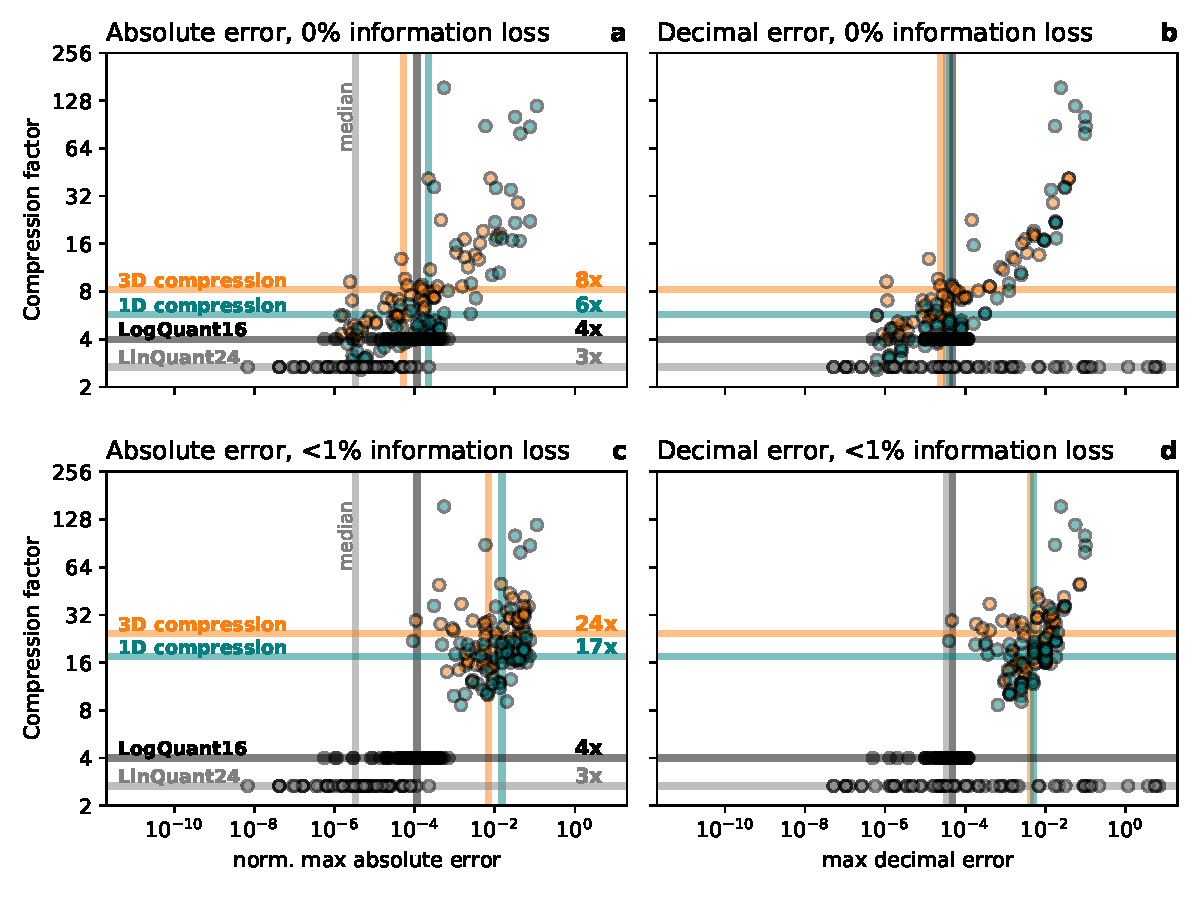
\includegraphics[width=1\textwidth]{Figures/compression/compression_error.pdf}
	\caption{\textbf{Compression factors versus compression errors.} The maximum absolute and decimal error
	for 24-bit linear and 16-bit logarithmic quantization (LinQuant24, LogQuant16) with 1-dimensional round+lossless
	and 3-dimensional Zfp compression. Every marker represents for one variable the global maximum of the \textbf{a, c}
	normalised absolute error, \textbf{b, d} decimal error for \textbf{a, b} 100\% preserved information, and \textbf{c, d}
	 99\% preserved information. The geometric mean of compression factors over all variables is given as horizontal lines.
	 The median of the errors across all variables is given as vertical lines.}
	\label{fig:compression_error}
\end{figure}

Compressing all variables in CAMS and comparing error norms reveals the advantages of the 1D round+lossless method
compared to the 24-bit linear quantization technique currently in use (Fig. \ref{fig:compression_error}). The maximum decimal
errors (see section \ref{sec:error_norms}) are smaller for many variables due to the logarithmic distribution of floating-point numbers.
Some variables are very compressible (>60x) due to many zeros in the data, which is automatically made use of in the lossless compression.
Compression factors are between 3x and 60x for most variables, with a geometric mean of 6x when preserving 100\% of information.
Accepting a 1\% information loss the geometric mean reaches 17x, which is the overall compression factor for the entire CAMS data
set with this method when compared to data storage with 64 bits per value.

Furthermore, the 24-bit linear quantization could be replaced by a 16-bit logarithmic quantization, as the mean and absolute errors
are comparable. The decimal errors are often even lower and naturally bound in a logarithmic quantization despite fewer available bits.

\begin{figure}[tbhp]
	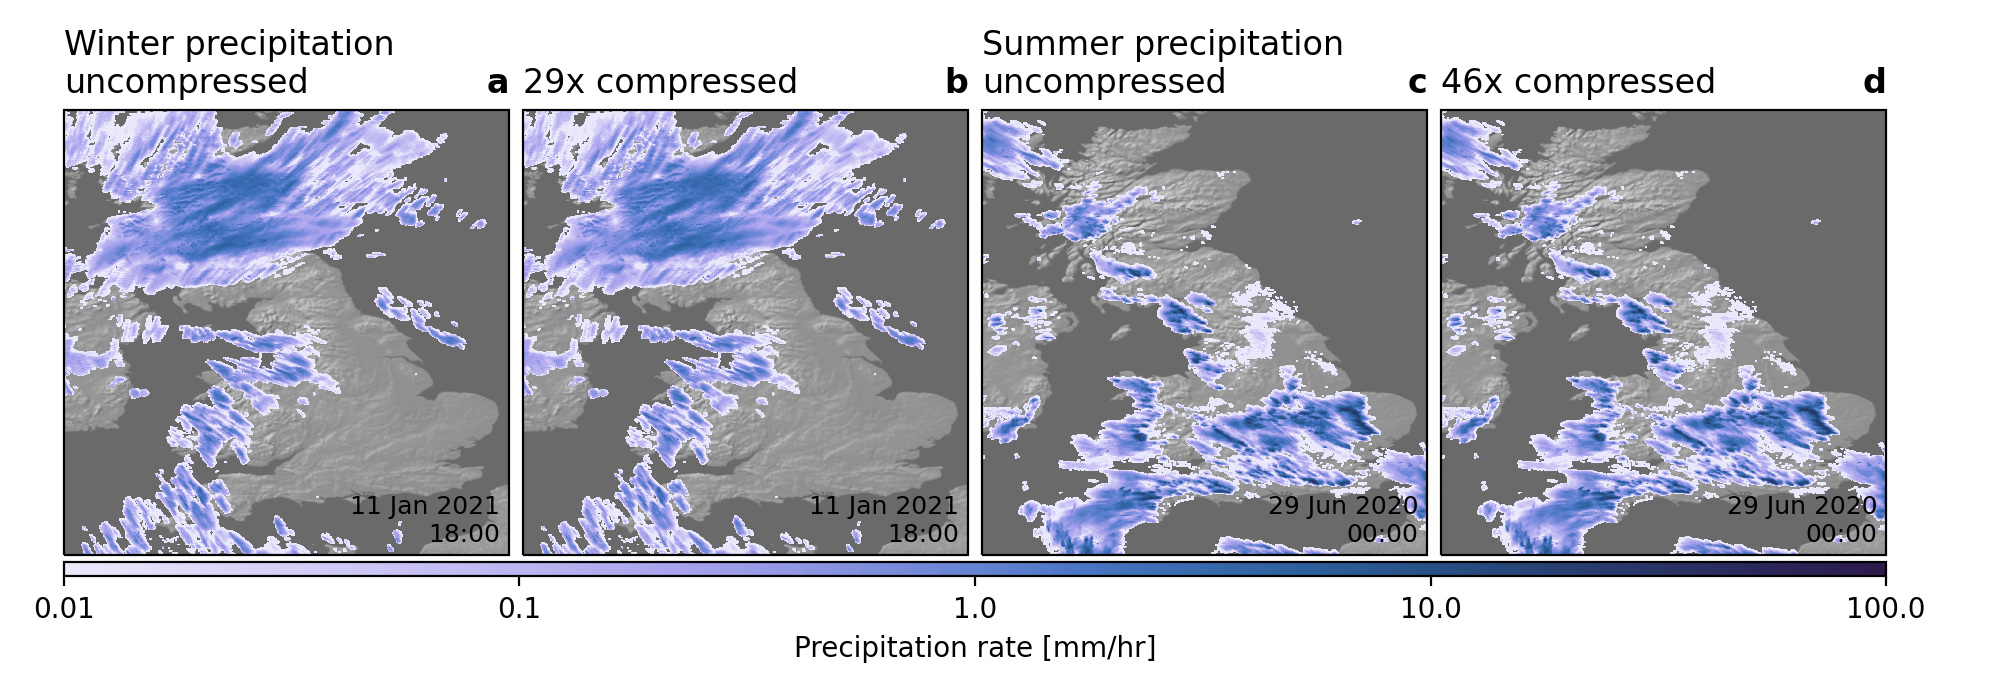
\includegraphics[width=1\textwidth]{Figures/compression/precipitation_compression.png}
	\caption{\textbf{Compression of radar-based observations of precipitation over Great Britain. a}
	Precipitation for the hour preceding 18:00 UTC on 11 Jan 2021 from the UK MetOffice NIMROD data at about 1km
	horizontal resolution. \textbf{b} as a but the data was compressed preserving 99\% of real information achieving
	compression factors of 29x relative to 64 bit. \textbf{c} and \textbf{d} as \textbf{a} and \textbf{b} but for 00:00 UTC
	on 29 Jun 2021 and achieving compression factors of 46x.}
	\label{fig:precipitation}
\end{figure}

\begin{figure}[tbhp]
	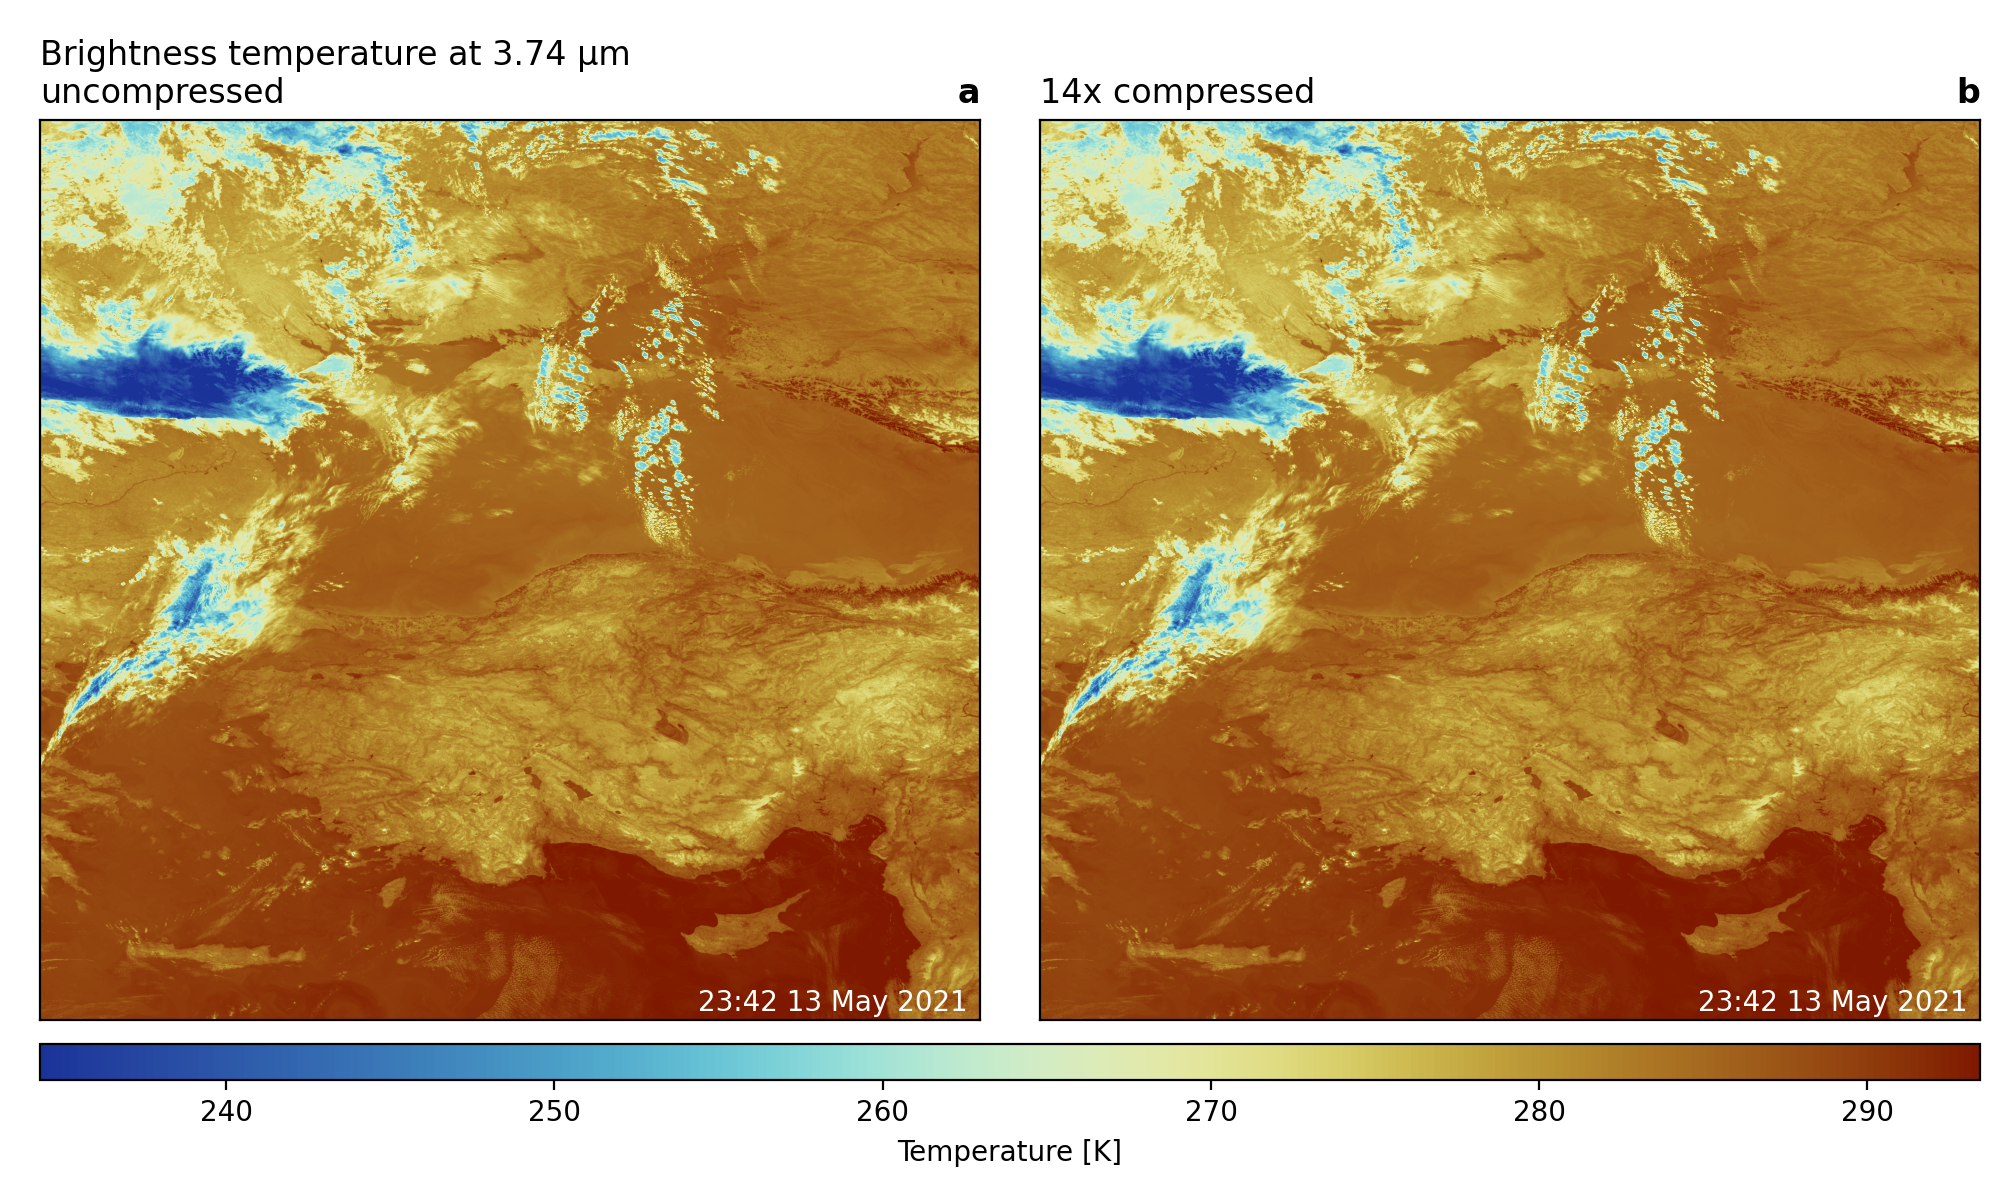
\includegraphics[width=1\textwidth]{Figures/compression/brightness_temp.png}
	\caption{\textbf{Compression of satellite-based observations of brightness temperature over the
	Black Sea and Turkey. a} Brightness temperature measured by the 3.74\textmu m (I4) channel of
	the VIIRS sensor on board the Suomi-NPP satellite at about 300m horizontal resolution on
	the 13 May 2021. \textbf{b} as \textbf{a} but the data was compressed preserving 99\% of
	real information with the round+lossless method achieving compression factors of 14x
	relative to 64 bit.}
	\label{fig:brightness_temp}
\end{figure}

\begin{figure}[tbhp]
	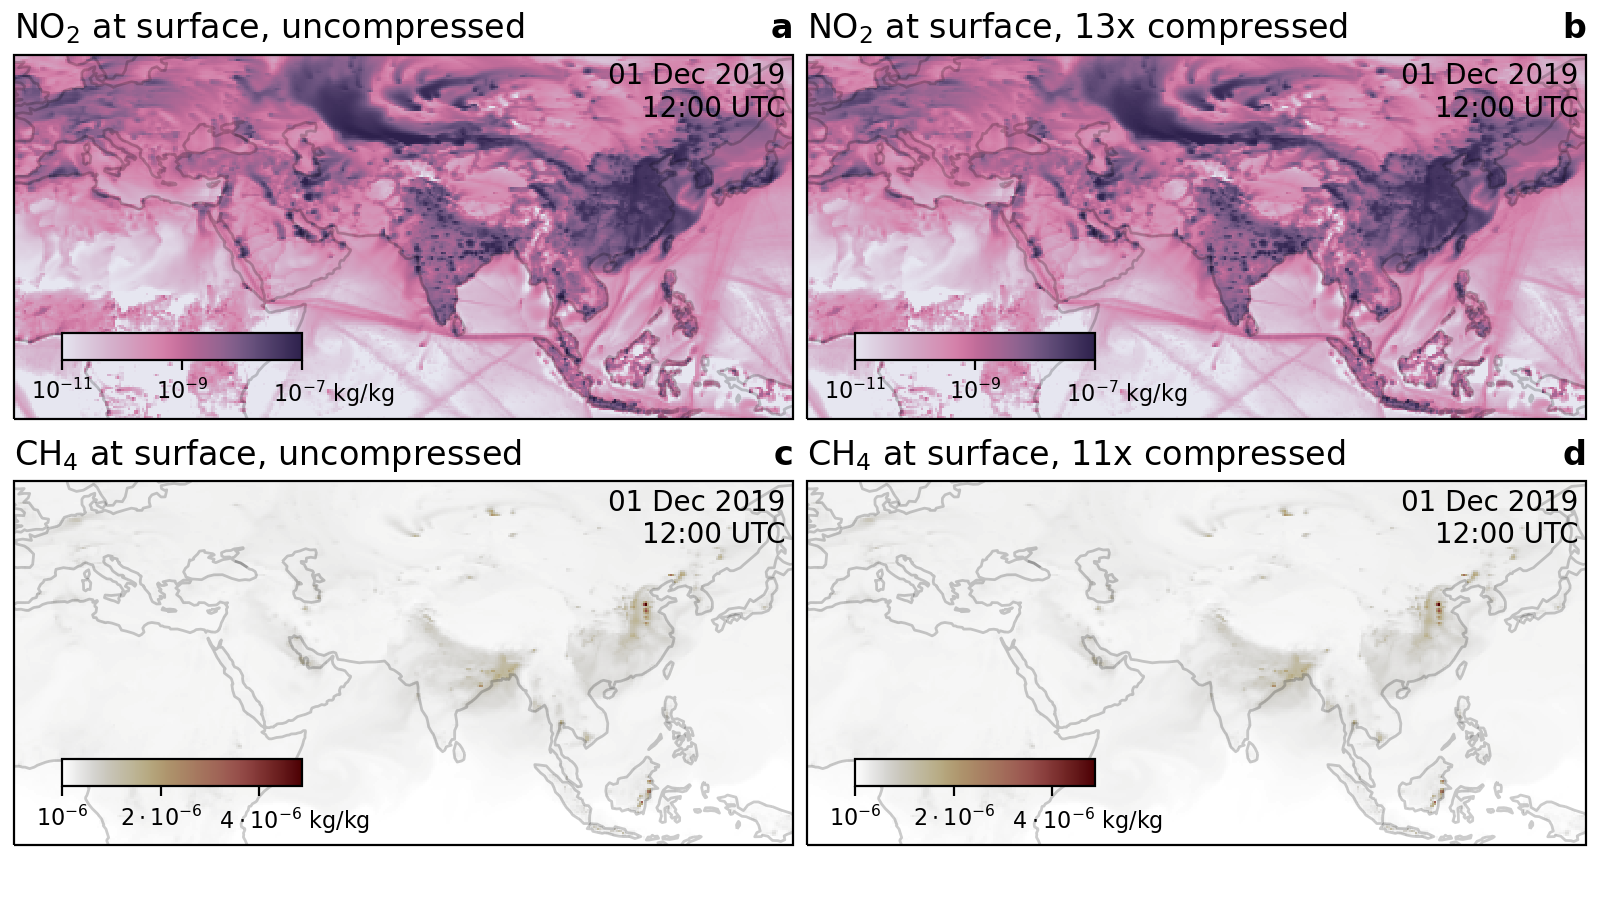
\includegraphics[width=1\textwidth]{Figures/compression/methane_no2_surface.png}
	\caption{\textbf{Compression of nitrogen dioxide (NO\textsubscript{2}) and methane (CH\textsubscript{4}) at the surface. a}
	Surface NO\textsubscript{2} concentrations preliminary result from fossil fuel combustion. \textbf{b} Surface CH\textsubscript{4}
	concentrations often include point sources, such as here in East China, East India and East Borneo. 
	\textbf{b,d} as \textbf{a,c} but compressed preserving 99\% of information achieving a compression factor of 13x, 11x,
	respectively.}
	\label{fig:methane_no2}
\end{figure}


A broad applicability of the bitwise real information content analysis for compression is tested with further data sets:
Radar-based observations of precipitation over Great Britain are similarly compressible using the same method
(Fig. \ref{fig:precipitation}) and so are satellite measurements of brightness temperature with a very high resolution
of about 300m horizontally (Fig. \ref{fig:brightness_temp}). Even for anthropogenic emissions of methane or nitrogen
dioxide similar compression results are obtained, despite limited spatial correlation of point sources (Fig. \ref{fig:methane_no2}).
The bitwise real information content in this case is largely determined by the smooth background concentrations and
therefore still sufficiently high to preserve the point sources. 

In an operational setting we recommend the following workflow: First, for each variable the bitwise real information
content is analysed from a representative subset of the data. Representative is, for example, a single time step for
subsequent time steps if the statistics of the data distribution are not expected to change. From the bitwise real information
the number of mantissa bits to preserve 99\% of information is determined  (the \emph{keepbits}). Second, during the simulation the
arrays that will be archived are rounded to the number of keepbits (which are held fixed) and compressed. The first step
should be done offline, meaning once in advance of a data-producing simulation. Only the second step has to be performed
online, meaning every time data is archived. 

\begin{figure}[tbhp]
	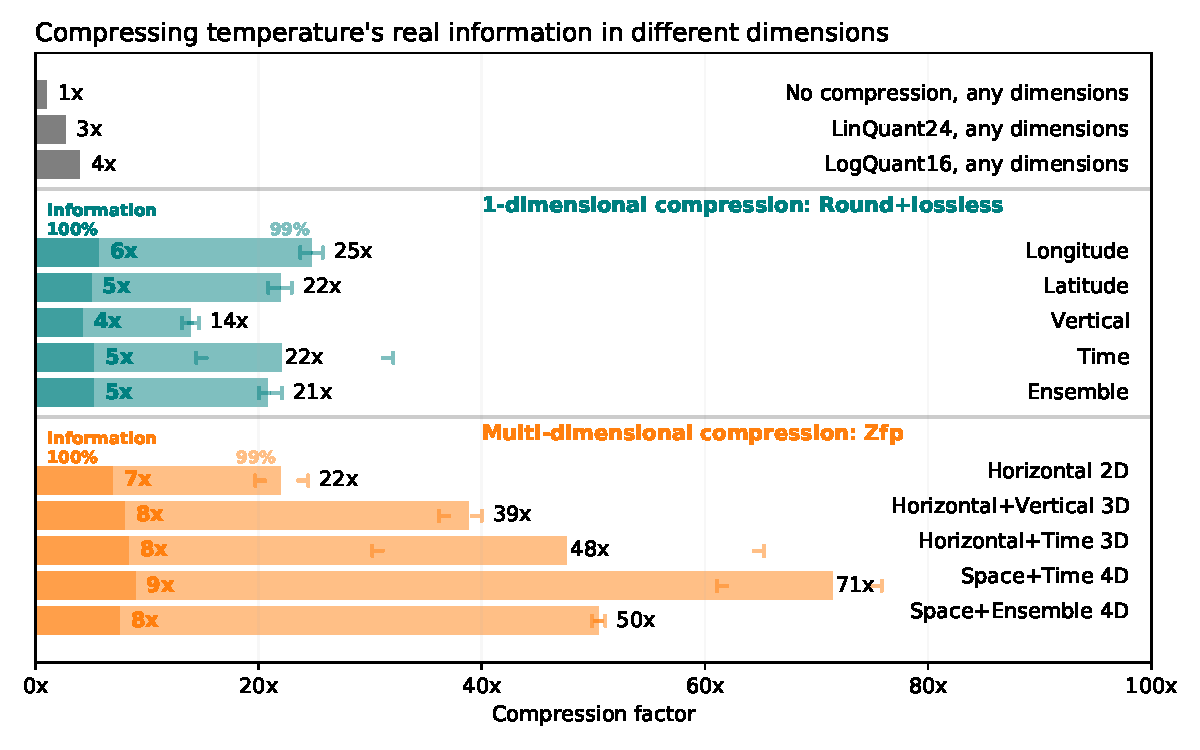
\includegraphics[width=1\textwidth]{Figures/compression/compressfac_comparison.pdf}
	\caption{\textbf{Multidimensional compression allows for higher compression factors.}
	\mbox{1-dimensional} compression (round+lossless) of temperature reaches at most 25x when preserving 99\% 
	of real information with the round+lossless method, whereas 71x is reached with 4-dimensional (4D)
	space-time compression using Zfp compression. Preserving 100\% of information considerably lowers
	the compression factors to 4-9x. Error brackets represent the min-max range of compression when
	applied to various data samples.}
	\label{fig:compressfac_comparison}
\end{figure}

The presented round+lossless compression technique separates the lossy removal of false information and the actual lossless
compression. This provides additional flexibilities as any lossless compressor can be used and application-specific choices can
be made regarding availability, speed and resulting file sizes. However, most general-purpose lossless compression algorithms
operate on bitstreams and require multidimensional data to be unravelled into a single dimension. Multidimensional correlation
is therefore not fully exploited in this approach.

We extend the ideas of information-preserving compression to modern multidimensional compressors. The analysis of the bitwise
real information content leads naturally to the removal of false information via rounding in the round+lossless method. For other
lossy compressors, however, the separation of real and false information has to be translated to the precision options of such
compressors. While such a translation is challenging in general, we present results from combining the bitwise real information
analysis with one modern multidimensional compressor in the next section.

\begin{figure}[tbhp]
	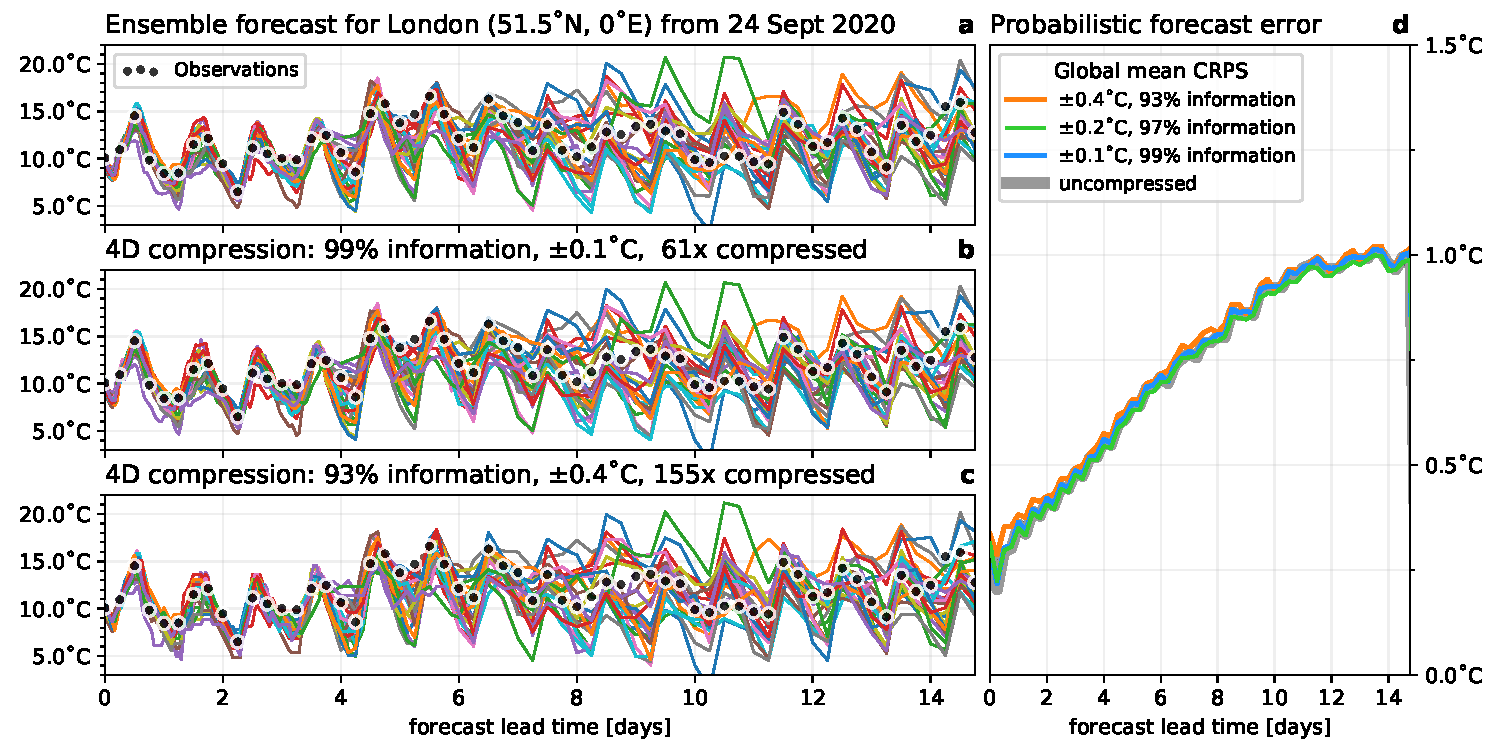
\includegraphics[width=1\textwidth]{Figures/compression/ensemble_forecast.pdf}
	\caption{\textbf{Verification of an ensemble forecast with the probabilistic forecast error based on ensemble data
	with and without compression. a} 25-member uncompressed ensemble forecast (lines) of surface temperature
	in London, UK from 24 Sept 2020 up to 15 days ahead. \textbf{b} as a but the data was compressed in 4-dimensional
	(4D) space-time with Zfp, preserving 99\% of real information. \textbf{c} as \textbf{b} but only preserving 93\% of real
	information. \textbf{d} Probabilistic forecast error (continuous ranked probability score, CRPS) for various levels of
	preserved information in the compression. The CRPS does not increases relative to the uncompressed reference for
	more than 93\% of preserved information.}
	\label{fig:ensemble_forecast}
\end{figure}

\subsection{Multidimensional climate data compression}

Modern compressors have been developed for multidimensional floating-point arrays
\citep{Lindstrom2006,Di2016,Ballester-Ripoll2020,Zhao2020,vonLarcher2019}, which compress in
several dimensions simultaneously. We will compare the 1D round+lossless compression to Zfp, a modern compression
algorithm for two to four dimensions \citep{Lindstrom2014,Pinard2020a,Poppick2020,Hammerling2019}.
Zfp divides a $d$-dimensional array into blocks of $4^d$  values (i.e. the edge length is 4), which allows to
exploit the correlation of climate data in up to 4 dimensions. To extend the concept of information-preserving
compression to modern compressors like Zfp, the bitwise real information is translated to the precision options of Zfp
(more details in section \ref{sec:compression_methods_compression}).

Multidimensional compression imposes additional inflexibilities for data retrieval: Data is compressed and decompressed
in larger chunks, which can increase the load on the data archive. For example, if the data is compressed across the time
dimension, data of several time steps have to be downloaded and decompressed although only data from a single time
step might be requested. Downloads from an archive might therefore increase if the data chunking is not well suited to
typical data requests from users. 

For 1D compression the compressibility varies with the dimension: Longitude (i.e. in the zonal direction) is more compressible,
reaching 25x for temperature at 99\% preserved information, than compressing in the vertical which yields only 14x
(Fig. \ref{fig:compressfac_comparison}). This agrees with the predominantly zonal flow of the atmosphere as spatial
correlation in the zonal direction is usually highest. For a constant number of retained mantissa bits, higher resolution
in the respective dimensions increases the compressibility as also the correlation in adjacent grid points increases
(Fig. \ref{fig:information_resolution} and \ref{fig:information_correlation}).

For multidimensional compression it is generally advantageous to include as many highly correlated dimensions as possible.
In that sense, including the hourly-resolved forecast lead time instead of the vertical dimension in 3D compression yields
higher compression factors. 4D space-time compression is the most efficient, reaching 60-75x at 99\% preserved information.
For temperature this is equivalent to a median absolute error of 0.1\textdegree{}C (Fig. \ref{fig:map_roundlossless_zfp}b).

\begin{figure}[tbhp]
	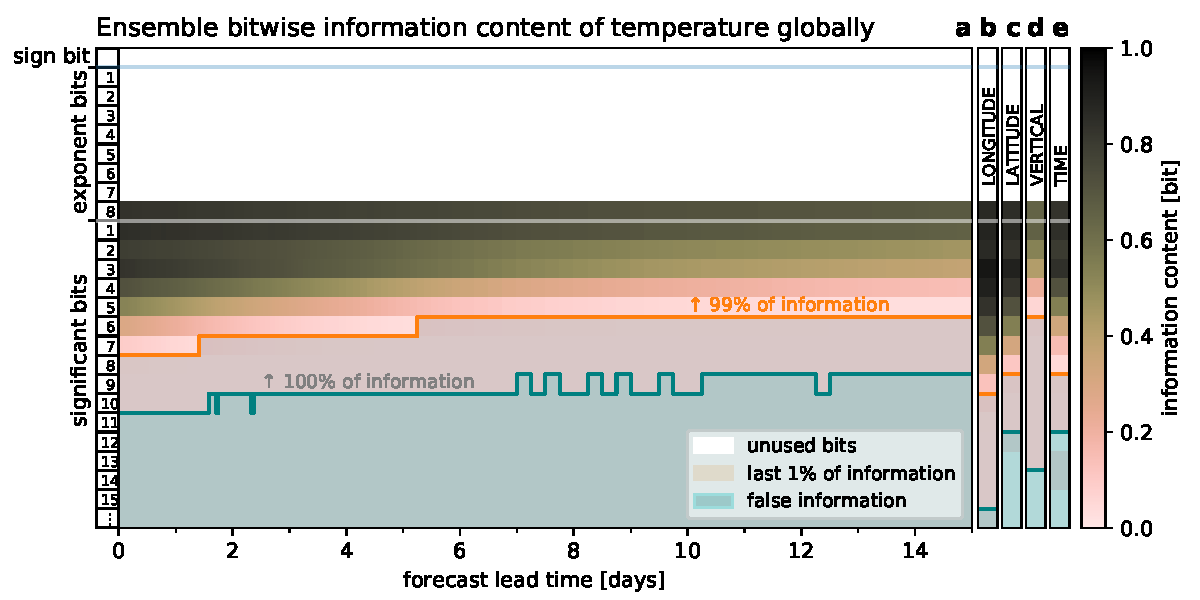
\includegraphics[width=1\textwidth]{Figures/compression/ensemble_information.pdf}
	\caption{\textbf{Bitwise real information content for temperature in various dimensions. a} ensemble, \textbf{b} longitude,
	\textbf{c} latitude, \textbf{d} vertical and \textbf{e} forecast lead time. The ensemble information effectively encodes the
	ensemble mean, which is less information than in most other dimensions. Longitude, latitude and forecast lead time
	have the highest total information which should be preserved in compression. The ensemble information decreases
	over time as the ensemble spread increases (Fig. \ref{fig:ensemble_forecast}).}
	\label{fig:ensemble_information}
\end{figure}

Compressing the entire CAMS dataset in the three spatial dimensions with Zfp while preserving 99\% of the information yields
an overall compression factor of 24x (Fig. \ref{fig:compression_error}). Maximum absolute error and decimal errors are for
most variables very similar to 1D round+lossless (see Fig. \ref{fig:compression_error_distribution} and section
\ref{sec:compression_methods_compression} for a discussion why they are not identical), providing evidence that a
multidimensional compression is preferable for higher compression factors. 

Due to the limited meaning of error norms in the presence of uncertainties in the uncompressed reference data, the forecast
error is assessed to quantify the quality of compressed atmospheric data. The continuous ranked probability score
(CRPS, \cite{Matheson1976,Hersbach2000,Zamo2018}),
a generalisation of the root-mean-square error for probabilistic forecasts, is evaluated for global surface temperature using observations
every 6 hours as truth (Fig. \ref{fig:ensemble_forecast}). Compared to the uncompressed data, no significant increase of the CRPS forecast error 
occurs for individual locations or globally at 99\% and 97\% preserved information. The usefulness for the end user of the global temperature
forecast is therefore unaltered at these levels of preserved information in the compression. Contrarily, with an information loss larger than
5\% the CRPS forecast error starts to increase, while large compression factors beyond 150x are achieved.

\subsection{A Turing test for data compression}

In numerical weather predictions, progress in the development of global weather forecasts is often assessed using a set of error metrics,
summarised in so-called \emph{score cards}. These scores cover important variables in various large scale regions, such as 2m-temperature
over Europe or horizontal wind speed at different vertical levels in the Southern Hemisphere. With a similar motivation as in \cite{Baker2019},
we suggest assessing the efficiency of climate data compression using similar scores, which have to be passed similar to a Turing test
\citep{Baker2016,Turing1950}.
The compressed forecast data should be indistinguishable from the uncompressed data in all of these score tests, or at least indistinguishable
from the current compression method while allowing higher compression factors. 

Many score tests currently in use represent area-averages (such as Fig. \ref{fig:ensemble_forecast}d), which would also be passed with
coarse-grained data — reducing the horizontal resolution from 10km to 20km, for example, yields a compression factor of 4x. It is therefore
important to include resolution-sensitive score tests such as the maximum error in a region. While a compression method either passes or
fails such a data compression Turing test, there is additional value in conducting such a test. Evaluating the failures will highlight problems
and evaluating the passes may identify further compression potential.

\section{Discussion}
\label{sec:compression_discussion}

While weather and climate forecast centres produce very large amounts of data, especially for future cloud and storm-resolving models,
only the real information content in this data should be stored. We have here presented a methodology to identify real and false information
in atmospheric, and more generally, climate data. This novel information-preserving compression relies on the removal of false information
via rounding and can then be used in combination with any lossless compression algorithm. Applied to CAMS data we show that a high
compressibility can be achieved without increasing the forecast error. The entire data set is 17x smaller in the compressed form when
compared to 64-bit values but preserves 99\% of the real information. This is about 6-times more efficient when compared to the
current compression method.

Alternatively, the analysis of the bitwise real information content can be used to inform multidimensional compressors. Ideally, climate data
compression should exploit correlation in as many dimensions as possible for highest compression factors. The most important dimensions
to compress along are longitude, latitude and time, which provide the highest compressibility. With Zfp we achieve factors of 60-75x for
4D space-time compression of temperature while preserving 99\% of real information and without increasing forecast errors. Using the three
spatial dimensions the entire set of variables in CAMS data can be compressed by 24x equivalently.

No additional uncertainty measure has to be assumed for the distinction of real and false information presented here. The uncertainty of a variable
represented in a data array is directly obtained from the distribution of the data itself. Most lossy compression techniques leave the choice of
precision to the user, which may lead to subjective choices or the same precision for a group of variables. Instead, our suggestion that
99\% of information should be preserved may be altered by the user, which will implicitly determine the required precision for each variable individually. 

To be attractive for large data sets, a compression method should enable compression as well as decompression at reasonable speeds.
ECMWF produces data at about 2GB/s, including CAMS which creates about 15 MB/s. Data on ECMWF’s archive is compressed once,
but downloaded on average at 120 MB/s by different users, such that both high compression and decompression speeds are important.
The (de)compression speeds obtained here are all at least 100MB/s single-threaded, but faster speeds
are available in exchange for lower compression factors (Fig. \ref{fig:compression_speed}). The real information is only analysed once
and ultimately independent of the compressor choice.

Lossy compression inevitably introduces errors compared to the uncompressed data. Weather and climate forecast data, however,
already contains uncertainties which are in most cases larger than the compression error. For example, limiting the precision of
surface temperature to 0.1\textdegree{}C (as shown in Fig. \ref{fig:map_roundlossless_zfp}b) is well below the average forecast error
(Fig. \ref{fig:ensemble_forecast}d) and also more precise than the typical precision of 1\textdegree{}C presented to end users of a
weather forecast. Reducing the precision to the real information content does not just increase compressibility but also helps to
directly communicate the uncertainty within the data set — an important, often neglected, information by itself.

Satisfying requirements on size, precision and speed simultaneously is an inevitable challenge of data compression. As the precision
can be reduced without losing information, we revisit this trade-off and propose an information-preserving compression. While current
archives likely use large capacities to store random bits, the analysis of the bitwise real information content is essential towards
efficient climate data compression.

\newpage
\section{Appendix}
\begin{table}[htbp]
	\center
	\footnotesize
	\begin{tabular}{l | l | l | l | l | l}
	\textbf{Name} & \textbf{Code} & \textbf{Unit} & \textbf{Name} & \textbf{Code} & \textbf{Unit} \\
	\hline
	\multicolumn{3}{l}{\textbf{Aerosols}} & \multicolumn{3}{l}{\textbf{Carbon oxides}}  \\
	Aerosol optical thickness 532nm & aott532 & 1 & Carbon dioxide & co2 & kg/kg \\
	Anthropogenic aot532 & aaot532 & 1 & Carbon monoxide & co & kg/kg \\
	Natural aot532 & naot532 & 1 &  \multicolumn{3}{l}{\textbf{Clouds and water}} \\
	Backscatter from ground at 1064nm & aergnd1064 & m\textsuperscript{-1}sr\textsuperscript{-1} & Fraction of cloud cover & cc &1 \\
Backscatter from ground at 355nm & aergnd355 & m\textsuperscript{-1}sr\textsuperscript{-1} & Cloud ice water & ciwc & kg/kg \\
Backscatter from ground at 532nm & aergnd532 & m\textsuperscript{-1}sr\textsuperscript{-1} & Cloud liquid water & clwc & kg/kg \\
Backscatter from top of atm at 1064nm & aertoa1064 & m\textsuperscript{-1}sr\textsuperscript{-1} & Specific rain water & crwc & kg/kg \\
Backscatter from top of atm at 532nm & aertoa355 & m\textsuperscript{-1}sr\textsuperscript{-1} & Specific snow water & cswc & kg/kg \\
Backscatter from top of atm at 532nm  & aertoa532 & m\textsuperscript{-1}sr\textsuperscript{-1} & Specific humidity & q & kg/kg \\
Aerosol extinction coefficient at 1064nm & aerext1064 & m\textsuperscript{-1} &  \multicolumn{3}{l}{\textbf{Methane}} \\
Aerosol extinction coefficient at 355nm & aerext355 & m\textsuperscript{-1} & Methane & ch4 & kg/kg \\
Aerosol extinction coefficient at 532nm & aerext532 & m\textsuperscript{-1} & Methane (chemistry) & ch4\_c & kg/kg \\
Aerosol type 2 source/gain accum. & aergn02 & kg/m\textsuperscript{2} & Methane loss rate & kch4 & s\textsuperscript{-1} \\
Aerosol type 7 source/gain accum. & aergn07 & kg/m\textsuperscript{2} & \multicolumn{3}{l}{\textbf{Alkanes or alcohols}} \\
Aerosol type 9 source/gain accum. & aergn09 & kg/m\textsuperscript{2} & Ethene & c2h4 & kg/kg \\
Aerosol type 10 source/gain accum. & aergn10 & kg/m\textsuperscript{2} & Ethanol & c2h5oh & kg/kg \\
Aerosol type 11 source/gain accum. & aergn11 & kg/m\textsuperscript{2} & Ethane & c2h6 & kg/kg \\
Aerosol large mode mixing ratio & aerlg & kg/kg & Propane & c3h8 & kg/kg \\
Sea salt (0.03-0.5\textmu m) & aermr01 & kg/kg & Isoprene & c5h8 & kg/kg \\
Sea salt (0.5-5\textmu m) & aermr02 & kg/kg & Acetone & ch3coch3 & kg/kg \\
Sea salt (5-20\textmu m) & aermr03 & kg/kg & Methanol & ch3oh & kg/kg \\
Dust aerosol (0.03-0.55\textmu m) & aermr04 & kg/kg & Methyl peroxide & ch3ooh & kg/kg \\
Dust aerosol (0.55-0.9\textmu m) & aermr05 & kg/kg & Hydrogen peroxide & h2o2 & kg/kg \\
Dust aerosol (0.9-20\textmu m) & aermr06 & kg/kg & Formaldehyde & hcho & kg/kg \\
Hydrophilic organic matter & aermr07 & kg/kg & Formic acid & hcooh & kg/kg \\
Hydrophobic organic matter & aermr08 & kg/kg & Nitric acid & hno3 & kg/kg \\
Hydrophilic black carbon & aermr09 & kg/kg & Hydroperoxy radical & ho2 & kg/kg \\
Hydrophobic black carbon & aermr10 & kg/kg & Hydroxyl radical & oh & kg/kg \\
Sulphate aerosol & aermr11 & kg/kg & Aldehyde & ald2 & kg/kg \\
Nitrate fine mode & aermr16 & kg/kg &  \multicolumn{3}{l}{\textbf{Nitrogen and sulfur oxides}} \\
Nitrate coarse mode & aermr17 & kg/kg & Nitrogen dioxide & no2 & kg/kg \\
Ammonium aerosol & aermr18 & kg/kg & Nitrogen monoxide & no & kg/kg \\
 \multicolumn{3}{l}{\textbf{Others}}  & Sulphur dioxide & so2 & kg/kg \\
Olefins & ole & kg/kg &  \multicolumn{3}{l}{\textbf{Ozone}}  \\
Organic nitrates & onit & kg/kg & Ozone mixing ratio 2 & go3 & kg/kg \\
Peroxyacetyl nitrate & pan & kg/kg & Ozone mixing ratio 1 & o3 & kg/kg \\
Paraffins & par & kg/kg & Stratospheric ozone & o3s & kg/kg
        \end{tabular}
	\caption{\textbf{Variables, their codes and units in the Copernicus Atmospheric Monitoring Service.}}
	\label{tab:cams_abbreviations}
\end{table}

